% !TEX root = ../../thesis.tex

\section{Nonlinear Secure Estimation \label{sec:nonlinear_se}}
%\begin{abstract}
%\textcolor{black}{We focus on securely estimating the state of a nonlinear dynamical system from a set of corrupted measurements for two classes of nonlinear systems, and propose a technique which enables us to perform secure state estimation for those systems. We then illustrate how the proposed nonlinear secure state estimation technique \textcolor{black}{can be used to perform estimation} in the cyber layer of interconnected power systems under cyber-physical attacks and communication failures. In particular, we focus on an interconnected power system comprising several synchronous generators, transmission lines, loads, and energy storage units, and propose a secure estimator that allows us to securely estimate the dynamic states of the power network. Finally, we numerically demonstrate the effectiveness of the proposed secure estimation algorithm, and show that the algorithm enables the cyber layer to accurately reconstruct the attack signals.}
%\end{abstract}


%!TEX root = ../../thesis.tex

\section{Introduction}
\label{sec:Introduction}
%According to \cite{Perez-Lombard:2008aa}, residential and commercial buildings account for up to 40\% of the total electricity consumption in developed countries, with an upward trend. Heating, ventilation and air-conditioning (HVAC) systems are a major source of this consumption \cite{USenergy:2017}. %, ~35% of energy use in commercial buildings is for heating, cooling and ventilation.
%Nevertheless, their power consumption can be flexibly scheduled without compromising occupant comfort, due to the thermal capacity of buildings. As a result, HVAC systems have become the focal point of research, with the goal of utilizing this source of consumption flexibility. From the point of view of energy efficiency, researchers have studied optimization of building control in order to minimize power consumption \cite{Siroky:2011aa, Parisio:2014aa}.  
%More recently, it has been proposed to engage buildings in supporting the supply quality of electricity and the grid stability, by participating in the regulation of electricity's frequency \cite{Balandat:2014contractdesign, Lin:2015exp, Vrettos:2014aggregation, Baccino:2014aa}.
%
%
%All of the above research activities are based on a valid mathematical model describing the thermal behavior of buildings. 

Traditionally, buildings have been modeled with high-dimensional physics-based models such as resistance-capacitance (RC) models \cite{Maasoumy:2014ab, Sun, David, Hao_multizone}, TRNSYS \cite{Duffy:2009aa} and EnergyPlus \cite{Zhao2013EP}. These models are motivated by the thermodynamics of the building and explicitly model the heat transfer between components of the buildings. The advantage of such models is their high granularity of temperature modeling, but a drawback is their high dimensionality which makes them computationally expensive. 
Although there has been extensive work on model reduction, this remains to be a non-trivial task. A large body of this work focuses on linear models, whereas physics-based models for commercial buildings with a variable air volume (VAV) HVAC system are bilinear in nature. Furthermore, existing model reduction techniques often result in a loss of interpretability of states \cite{Dobbs:2012aa} and a significant increase in the model's prediction error \cite{Goyal:2012modelreduction}. 

Motivated by these shortcomings, a new direction of research attempts to identify lower-dimensional, data-driven models, e.g. with Input-Output models \cite{Lin:2015exp} and semiparametric regression \cite{Aswani:2012aa}. The purpose is to alleviate the computational complexity in expense for coarser and less accurate temperature predictions.


%The contribution of this paper is two-fold. First, we aim to improve existing
%data-driven model identification techniques. Unlike \cite{Radecki:2012aa}, \cite{Radecki:2013ab}, who model the evolution of the building's energy consumption without a specific control input, we identify a model for temperature evolution in multiple building zones that is amenable to control design, i.e. with airflows as inputs. Our model also differs from that in \cite{Aswani:2012aa}, which uses HVAC supply air temperature as the single control input, resulting in a simpler identification problem but on the other hand, offers less flexibility in control.

In this chapter, we propose both a physics-based method and a data-driven method to identify models of a multi-zone building, that is easy to implement with the building in regular operation, and captures internal gains such as occupancy, without the need of additional instruments like carbon dioxide sensors.
Our procedures use excitation experiments that actively perturb the building and generate data that can be used for more accurate parameter identification.

More importantly, we perform a \textit{quantitative comparison} of the data-driven and physics-based models in terms of open-loop prediction accuracy and closed-loop control strategies, based on the \textit{same testbed} (the entire floor of an office building). % using \textit{experimental data} collected from the building, as opposed to simulated data. 
We conclude that a low-dimensional data-driven model is suitable for building control applications, such as frequency regulation, due to its minor loss of prediction accuracy compared to high-dimensional physics-based models, but significant gain in computational ease. 
To the best of our knowledge, the extant body of literature has analyzed data-driven and physical models for the identification of temperature evolution in commercial buildings only in an isolated fashion (in particular not on the same testbed) \cite{Ma:2011aa}, \cite{Siroky:2011aa}, \cite{Lin:2015exp}, \cite{Qie}. In addition, some of these models were identified for fictitious buildings with synthetic data \cite{Cole:2013aa, Goyal:2013occupancy, David}, while others used experimental data collected under environments with little or no disturbance, e.g. without occupants \cite{Lin:2015exp}. Our work differs from these existing works in two aspects. First, we use experimental data to identify models for a multi-zone commercial building under regular operation, which is subject to significant disturbances such as occupancy. Second, although the existing literature mentions the differences between data-driven and physics-based models, the prevailing isolationist approach does not provide any quantitative comparison with respect to building control applications - a fact we would like to alleviate by juxtaposing a data-driven with a physics-based model.


%The remainder of this paper is organized as follows: In Section \ref{sec:Preliminaries}, we describe the testbed and the experimental data collected for our research. Section \ref{sec:Data_Driven_Model} presents the identification process for a purely data-driven model with semiparametric regression, followed by Section \ref{sec:Physics_Based_Model}, which details the procedure for identifying a physics-based model. Section \ref{sec:Comparison} then compares the performance of the data-driven model and the physics-based model under open-loop prediction accuracy and closed-loop energy efficient optimal control. We show that, despite the higher accuracy of the complex physics-based model compared to the low-dimensional data-driven model, the optimal control strategies with respect to HVAC operation cost while maintaining the thermal comfort of occupants is almost identical for both systems. We conclude in Section \ref{sec:Conclusion} with a summary of our current and intended future work.




%%%%%%%%%%%%%%%%%%%%%%%%%%%%%%%%%%%%%%%%%%%%%%%%%%%%%%%%%%%%%%%%%%%%%%%
%%%%%%%%%%%%%%%%%%%%%%%%%%%%%%%%%%%%%%%%%%%%%%%%%%%%%%%%%%%%%%%%%%%%%%%%


%\section{Error Correction: A Review}\label{sec:review}
%
%\textcolor{red}{May not be needed as it repeats what's in the linear SE section.}
%
%\subsection{Classical Error Correction}
%\textbf{Compressed Sensing:} Sparse solutions $x\in \mathbb{R}^n$, are sought to the following problem:
%\begin{equation}
%	\min_x %\norm{x}_0 \text{ subject to } b= Ax
%	\label{eq:CS}
%\end{equation}
%where $b \in \mathbb{R}^m$ are the measurements, and $A \in \mathbb{R}^{m\times n}~ (m \ll n)$ is a sensing matrix. 
%%$\norm{x}_0$ 
%denotes the number of nonzero elements of $x$. The following lemma provides a sufficient condition for a unique solution to (\ref{eq:CS}).
%
%%\textcolor{black}{in II.A., you reference [16] right before Lemma 1 and [18] inside Lemma 1.  This is confusing.  If you are referencing the form of Lemma 1 from [16] that is presented in [18] then you should be explicit about it.}
%%\textcolor{black}{I removed [18] here, but we cite it later in IIB before equation (5).}
%\begin{lem} (\hspace{1sp}\cite{Candes_Tao}) \label{lem:CS}
%If the sparsest solution to (\ref{eq:CS}) has $\norm{x}_0 = q$ and $m\ge 2q$ and all subsets of $2q$ columns of $A$ are full rank, then the solution is unique.
%\end{lem}
%\begin{pf}
%Suppose the solution is not unique. Therefore, there exists $x_1 \neq  x_2$ such that $Ax _1 = b$ and $Ax_2 = b$ where $\norm{x_1}_0 = \norm{x_2}_0 = q$. Then, $A(x_1 - x_2) = 0$ and $x_1 - x_2 \neq 0$. Since $\norm{x_1-x_2}_0 \leq 2q$ and all $2q$ columns of $A$ are full rank (i.e. linearly independent), it is impossible to have $x_1-x_2\neq 0$ that satisfies $A(x_1-x_2) = 0$. This contradicts the assumption.
%\end{pf}\qed
%
%
%%%%%%%%%%%%%%%%%%%%%%%%%%%%%%%%%%%%%%
%\textbf{The Error Correction Problem \cite{Candes_Tao}:} %\label{sec:error_correction}
%Consider the classical error correction problem: $y=Cx + e$ where $C\in \mathbb{R}^{l\times n}$ is a coding matrix $(l > n)$ and assumed to be full rank. We wish to recover the input vector $x \in \mathbb{R}^n$ from corrupted measurements $y$. Here, $e$ is an arbitrary and unknown sparse error vector. To reconstruct $x$, note that it is obviously sufficient to reconstruct the vector $e$ since knowledge of $Cx + e$ together with $e$ gives $Cx$, and consequently $x$ since $C$ has full rank \cite{Candes_Tao}. In \cite{Candes_Tao}, the authors construct a matrix $F$ which annihilates $C$ on the left, i.e.,  $FCx = 0$ for all $x$. Then, they apply $F$ to the output $y$ and obtain
%\begin{equation}
%	\tilde y = F (Cx + e) = Fe.
%\end{equation}
%Thus, the decoding problem can be reduced to that of reconstructing a sparse vector $e$ from the observations $\tilde y = Fe$. Therefore, by Lemma \ref{lem:CS}, if all subsets of $2q$ columns of $F$ are full rank, then we can reconstruct any $e$ such that $\| e \|_0 \leq q$.
%%We refer to a decoder that can correct $q$ errors as a $q$-error-correcting decoder.
%
%
%%%%%%%%%%%%%%%%%%%%%%%%%%%%%%%%%%%%%%
%\subsection{Secure Estimation for Linear Dynamical Systems \cite{David_Chang2} }
%
%%\textcolor{black}{II.B. seems like it should reference [11] -- is this the exact formulation in [11] or is it changed to suit the development here?  In any case, be explicit about this.}
%
%Consider the linear control system as follows:
%\begin{equation}
%\begin{aligned}
%&x(k+1)= A x(k) ,\\
%&y(k) = C x(k) + e(k)
%\end{aligned}
% \label{eq:system_model_se}
%\end{equation}
%where $x(k) \in \mathbb{R}^n $ and  $y(k) \in \mathbb{R}^p$ represent the states and outputs of the system at time $k$, respectively. $e(k) \in \mathbb{R}^p$ represents attack signals injected by malicious agents at the sensors, and the set of attacked sensors can change over time.
%
%Consider the problem of reconstructing the initial state $x(0)$ of the plant from the corrupted observations $y(k)$'s where $k=0,...,T-1$.
%Let $E_{q,T}$ denote the set of error vectors $\begin{bmatrix} e(0); ~ ...~  ;  e(T-1) \end{bmatrix}   \in  \mathbb{R}^{p\cdot T} $ where each $e(k)$ satisfies $\|e(k)\|_0 \leq q \leq p$. %$\lvert \textsf{supp}(e(k)) \rvert \le q \le p $.
%\begin{eqnarray} \label{eq:sys_err_corr}
%\begin{aligned}
%	Y &\triangleq \begin{bmatrix} y(0) \\ y(1) \\ \vdots \\ y(T-1) \end{bmatrix}
%		= \begin{bmatrix} Cx(0) + e(0)\\ CA x(0) + e(1) \\ \vdots \\ CA^{T-1} x(0) + e(T-1) \end{bmatrix} \\
%		& =
%		\begin{bmatrix} C \\ CA \\ \vdots \\ CA^{T-1} \end{bmatrix} x(0) + E_{q,T} \triangleq \Phi x(0) + E_{q,T}
%		\label{eq:decoder_Phi}
%\end{aligned}
%\end{eqnarray}
%where $Y \in \mathbb{R}^{p\cdot T}$ is a collection of corrupted measurements over $T$ time steps and $\Phi \in \mathbb{R}^{p\cdot T \times n}$. \textcolor{black}{We call $\Phi$ the $T$-step observability matrix of the system.} %\st{ if $B=0$ (i.e., $A = A_o$)}. \st{Since we consider secure estimation of adversarial attacks,}
%Here, we need to assume that $\operatorname{rank}(\Phi) = n$; otherwise, the system is unobservable and we cannot determine $x(0)$ even if there was no attack (i.e., $E_{q,T} = 0$).
%
%
%Inspired by the error correction techniques proposed in \cite{Candes_Tao} and \cite{David_Chang2}, we first determine the error vector $E_{q,T}$, and then solve for $x(0)$. %[We say this upfront, so readers know what to expect, and it may be less surprising when they see the second method?]  \st{We consider the error correction approach.}
%Consider the $QR$ decomposition of $\Phi \in \mathbb{R}^{p\cdot T \times n}$,
%\begin{eqnarray}
%	\Phi = \begin{bmatrix} Q_1 & Q_2 \end{bmatrix} \begin{bmatrix} R_1 \\ 0 \end{bmatrix} = Q_1 R_1
%\end{eqnarray}
%where $\begin{bmatrix} Q_1 & Q_2 \end{bmatrix} \in \mathbb{R}^{p\cdot T \times p\cdot T}$ is orthogonal, $Q_1 \in \mathbb{R}^{p\cdot T\times n}, Q_2 \in \mathbb{R}^{p\cdot T \times (p\cdot T-n)}$, and $R_1 \in \mathbb{R}^{n\times n}$ is a rank-$n$ upper triangular matrix.
%Pre-multiplying (\ref{eq:decoder_Phi}) by $\begin{bmatrix} Q_1 & Q_2 \end{bmatrix} ^\top$ gives:
%\begin{equation}
%	\begin{bmatrix} Q_1 ^\top \\ Q_2 ^\top \end{bmatrix} Y = \begin{bmatrix}R_1 \\ 0  \end{bmatrix} x(0) + \begin{bmatrix} Q_1 ^\top \\ Q_2^\top \end{bmatrix} E_{q,T}.
%	\label{eq:QR}
%\end{equation}
%We can compute $E_{q,T}$ by using the second block row:
%\begin{equation}
%	\tilde Y \triangleq Q_2^\top Y = Q_2^\top E_{q,T}
%	\label{eq:E_est}
%\end{equation}
%where $Q_2^\top \in \mathbb {R} ^{ (p\cdot T-n) \times p\cdot T}$.
%\textcolor{black}{From Lemma \ref{lem:CS}, (\ref{eq:E_est}) has a unique, $s$-sparse solution (where $s\le q\cdot T$) if all subsets of $2s$ columns (at most $2 q\cdot T$ columns) of $Q_2^\top$ are full rank. Therefore, we consider solving the following $l_1$-minimization problem:}
%\begin{equation}
%	\hat{E}_{q,T} = \arg \min_E \norm { E}_{l_1} \text{ subject to } \tilde Y = Q_2^\top E
%	\label{eq:solve_E}
%\end{equation}
%\textcolor{black}{Note that the $l_0$-minimization problem can be approximated by an $l_1$-minimization problem to give a convex decoder that is computationally feasible. Motivated by the problem of finding sparse decompositions of special signals in the field of mathematical signal processing, a series of studies \cite{tao11}-\!\cite{Tropp11} showed exact equivalence between the two programs $l_0$ and $l_1$ when the Restricted Isometry Property conditions are satisfied. For more information on the equivalence between the $l_1$-minimization problem and the $l_0$-minimization problem, we refer the reader to \cite{tao11}-\!\cite{Tropp11}.}
%
%
%
%
%%Clearly, this is a reasonable assumption if $(p\cdot T-n) \ge 2q\cdot T$.
%
%Now, given the vector $\hat{E}_{q,T}$, we can compute $x(0)$ from the first block row of (\ref{eq:QR}) as follows:
%\begin{equation}
%	x(0) = R_1^{-1} Q_1^\top (Y- \hat{E}_{q,T})
%	\label{eq:QR1}
%\end{equation}
%The following lemma provides the conditions under which the solution to (\ref{eq:QR1}) exists and is unique.
%%\textcolor{black}{Specifically, does Lemma 2 need a citation?} \textcolor{green}{I think we need a citation here}\textcolor{black}{This is a result proved in [11], is it OK to just cite [11] or do we need any other citations?}
%\begin{lem} \label{lem:EC}
%	$x(0) $ is the unique solution if all subsets of $2s$ columns of $Q_2 ^\top$ are linearly independent and $\Phi$ is full column rank. %Also, this condition is equivalent to $\| \Phi z \|_0 > 2s$ %$\lvert \textsf{supp}( \Phi z) \rvert > 2 s = 2 (q\cdot T)$
%%for all $z \in \mathbb{R}^n \backslash \{ 0 \}$.
%\end{lem}
%\begin{pf}
%By Lemma \ref{lem:CS} and noting that by definition the null space of $Q_2^\top$ equals the column space of $\Phi$. %For the second statement, we would like to show that the following are equivalent: \\
%\end{pf}\qed



%%%%%%%%%%%%%%%%%%%%%%%%%%%%%%%%%%%%%%%%%%%%%%%%%%%%%%%%%%%%%%%%%%%%%%%
%%%%%%%%%%%%%%%%%%%%%%%%%%%%%%%%%%%%%%%%%%%%%%%%%%%%%%%%%%%%%%%%%%%%%%%%
% !TEX root = ../../thesis.tex
\subsection{Secure Estimation for Nonlinear Systems}\label{sec:nonlinear_estimation}
Consider a nonlinear dynamical system given by
\begin{equation}\label{eq:sys_dynamics}
\begin{aligned}
	x(k+1) &= A x (k) + f\big(x(k),e(k)\big) + u(k) \\
	y(k) &= C x(k) + e(k)
\end{aligned}
\end{equation}
where $x(k)\in \mathbb{R}^n$ represents the state at time $k\in
\mathbb{N}$, $A \in \mathbb{R}^{n\times n}$, $f(x(k),e(k)): \mathbb{R}^n \times \mathbb{R}^p \rightarrow \mathbb{R}^n$ represent the system's dynamics, and $u(k) \in \mathbb{R}^n$ is a control input. $C \in \mathbb{R}^{p\times n}$ is the sensors' measurement matrix, $y(k) \in \mathbb{R}^p$ are the corrupted measurements at time $k\in\mathbb{N}$, and $e(k)\in \mathbb{R}^p$ represents attack signals injected by malicious agents at the sensors. \textcolor{black}{In general, at each time instant, the system dynamics can be a function of the received measurements $y(k)$ as well as the state of the system $x(k)$. Since $y(k)$ can be expressed as a function of $x(k)$ and $e(k)$ using the measurement equation, we consider $f(x(k),e(k))$ to be a function of both $x(k)$ and $e(k)$.}



Our goal is to reconstruct $x(k)$ in (\ref{eq:sys_dynamics}) by using the received measurements. Here, we do not assume the errors $e(k)$ follow any particular model. More precisely, the $i$-th element of $e(k)$ can take any value in $\mathbb{R}$. However, if sensor $i\in \{1,2,\cdots,p\}$ is not attacked, then necessarily the $i$-th element of $e(k)$ is zero. \textcolor{black}{The only assumption concerning the corrupted sensors is the number of sensors that are attacked or corrupted due to failures. Our analytical results characterize the number of errors that can be corrected by a decoder.}


Next, we focus on the problem of reconstructing state $x(k)$ for two classes of nonlinear systems. %\textcolor{black}

%\vspace{-0.2cm}
\subsection{Existence of Mapping Function with Error Correction}\label{map_1}
Let us assume that there exists a mapping function $g\big(y(k)\big): \mathbb{R}^p \rightarrow \mathbb{R}^n$ such that
\begin{equation}\label{eq:mapping1}
g\big(y(k)\big)=f\big(x(k),e(k)\big)~
\end{equation}
The mapping function $g\big(y(k)\big)$ enables us to transform the nonlinear system in (\ref{eq:sys_dynamics}) into a linear system for which the error correction technique introduced in Section \ref{sec:review} can be used to reconstruct the initial state $x(0)$. To do so, we first use (\ref{eq:sys_dynamics}) and (\ref{eq:mapping1}) to obtain $g\big(y(k)\big)=x(k+1)-A x(k)-u(k)$ for all $k$. We then construct a vector $Y$ as follows:
\begin{equation}\label{map_1_error_correction}
\begin{aligned}
	Y&=\begin{bmatrix} y(0) \\ y(1) - C \big(g(y(0))+ u(0)\big)  \\
	y(2) - C \big( A g(y(0)) + A u(0) + g(y(1) ) + u(1) \big) \\ \vdots   \\
	y(T-1) - C \big(A^{T-2} g(y(0)) + A^{T-2} u(0) + \cdots \big) \end{bmatrix}
	\\&= \begin{bmatrix} C \\ CA \\ CA^2 \\  \vdots \\ CA^{T-1}  \end{bmatrix} x(0) + \begin{bmatrix} e(0) \\ e(1) \\ e(2) \\ \vdots  \\ e(T-1)\end{bmatrix} = \Phi x(0) + E
\end{aligned}
\end{equation}
where $E=[e(0);e(1);\cdots;e(T-1)]\in \mathbb{R}^{p \cdot T}$ is the set of error vectors, and $\Phi=[C;CA;CA^2;\cdots;CA^{T-1}]$.
%\sout {\textcolor{black}{In order to reconstruct $x(0)$, we need to have $\text{rank}(\Phi) = n$; otherwise, we cannot determine $x(0)$ even if there were no attack.}
%\textcolor{black}{This may sound like $\text{rank}(\Phi) = n$ is the only condition needed to reconstruct $x(0)$?}}

We can now apply the error correction technique introduced in the previous section to the linear system in (\ref{map_1_error_correction}). While the proposed technique enables us to reconstruct the initial state $x(0)$ from a set of corrupted measurements, it might not always be possible to find such a mapping function. Next, we focus on a larger class of nonlinear systems, and use feedback linearization to transform the nonlinear system in (\ref{eq:sys_dynamics}) into a linear system.



%\vspace{-0.2cm}
\subsection{Feedback Linearization}
Let us assume that there exist mapping functions $g\big(y(k)\big)$ and $h_1\big(x(k)\big)$ (which are not necessarily linear), and a linear map $h_2\big(e(k)\big)$ such that:
\begin{equation}\label{eq:form_feedback}
f\big(x(k),e(k)\big)= g\big(y(k)\big) + h_1\big(x(k)\big) + h_2\big(e(k)\big)	
\end{equation}
where $g\big(y(k)\big): \mathbb{R}^p \rightarrow \mathbb{R}^n$, $h_1\big(x(k)\big): \mathbb{R}^n \rightarrow \mathbb{R}^n$, and $h_2\big(e(k)\big): \mathbb{R}^p \rightarrow \mathbb{R}^n$ are non-zero.
%Since we have a local feedback loop, we can consider a new input variable
Without loss of generality, we can choose the control input $u(k)$ such that $u(k)=-h_1 \big(x(k) \big)+v(k)$. \noindent \textcolor{black}{Note that the specific form of our control input does not mean that we cannot use the estimator in control applications. Here, $v(k)$ allows us to choose our control strategy in the desired way (e.g., LQG control).} By using this control input, we cancel out the nonlinear term $h_1\big(x(k)\big)$, and obtain:
\begin{equation}
\begin{aligned}
	g\big(y(k)\big) &= x(k+1) - A x(k) - v(k) - h_2\big(e(k)\big).\nonumber
\end{aligned}
\end{equation}
We can now construct a vector $Y$ as follows:
\begin{equation}
\begin{aligned}
	Y=&\begin{bmatrix} y(0) \\ y(1) - C \big(g(y(0)) + v(0) \big) \\
	y(2) - C \big( A g(y(0)) + Av(0)  + g(y(1))  + v(1) \big)\\ \vdots \\ y(T-1) - C \big(A^{T-2} g(y(0)) + A^{T-2} v(0) + \cdots \big) \end{bmatrix}  \\
	=&~\Phi x(0) +
	\begin{bmatrix} 0 \\ C h_2 \big(e(0) \big) \\ C A h_2 \big(e(0) \big) + C h_2 \big(e(1) \big)  \\ \vdots  \\ C A^{T-2} h_2 \big(e(0) \big)  \cdots \end{bmatrix}
\end{aligned}
\end{equation}
Note that $h_2(\cdot)$ is a linear map (i.e., $h_2 \big(e(k) \big) = H e(k)$ where $H \in \mathbb{R}^{n \times p }$). Hence, we obtain:
\begin{equation}\label{linear_feed}
\begin{aligned}
Y &= \Phi x(0) + \Psi E
\end{aligned}
\end{equation}
where matrices $\Phi \in \mathbb{R}^{p\cdot T \times n}$ and $\Psi \in \mathbb{R}^{p\cdot T \times p\cdot T}$ are as follows:
\begin{equation}
\begin{aligned}
\Phi=\begin{bmatrix} C \\ CA \\ CA^2 \\ \vdots \\ CA^{T-1} \end{bmatrix},
\Psi = \begin{bmatrix} I & & & &   \\
CH & I & & \\
CAH & CH & I & \\
\ddots & \ddots  &  \ddots &  \ddots & \\
CA^{T-2} H & \cdots & \cdots & \cdots & I
\end{bmatrix}.\nonumber
\end{aligned}
\end{equation}
We can now apply the error correction method introduced in Section \ref{sec:review} to the linearized system in (\ref{linear_feed}) and reconstruct $x(0)$ if the condition in Lemma \ref{lem:EC} is satisfied.



\begin{remark}
(Measurement Noise) In practice, the measurements are noisy so one cannot assume that the $Ax$ term in (\ref{eq:CS}) is known with arbitrary precision. More appropriately, we need to assume that one is given noisy measurement, i.e., $b = Ax + \epsilon$, where $\epsilon$ represents measurement noise. In \cite{Candes_Tao}, the authors prove that one can recover approximately sparse signals with an error at most proportional to the noise level. Alternatively, one can combine secure estimation with a KF to improve the secure estimator's performance for noisy measurements \cite{Hu:2016uav}: the KF filters out both occasional estimation errors by the secure estimator and noisy measurements.
\end{remark}


In this study, we focus on sensor attack within a noiseless framework. Next, we consider an interconnected power system with several synchronous generators, and illustrate how the proposed nonlinear state estimation approach can be applied for secure state estimation of dynamic states (i.e., generator' phase angles and rotors' speeds).

%%%%%%%%%%%%%%%%%%%%%%%%%%%%%%%%%%%%%%%%%%%%%%%%%%%%%%%%%%%%%%%%%%%%%%%
%%%%%%%%%%%%%%%%%%%%%%%%%%%%%%%%%%%%%%%%%%%%%%%%%%%%%%%%%%%%%%%%%%%%%%%%


% !TEX root = ../../thesis.tex

\section{Power System State Estimation}\label{sec:application}
We first introduce the physical layer model of an interconnected power system comprising several synchronous generators and buses, and then introduce a graph-theoretic model to describe the communication network which interconnects the wide-area and local controllers of the power system. Fig.~\ref{ps} illustrates the interactions between the physical and cyber layers in the system. Note that the components of the system and the notation used
in this figure will be introduced throughout this section. Finally, we introduce two categories of cyber attacks that can potentially corrupt measurements and degrade the system's performance.

\begin{figure*}[t]
\begin{center}
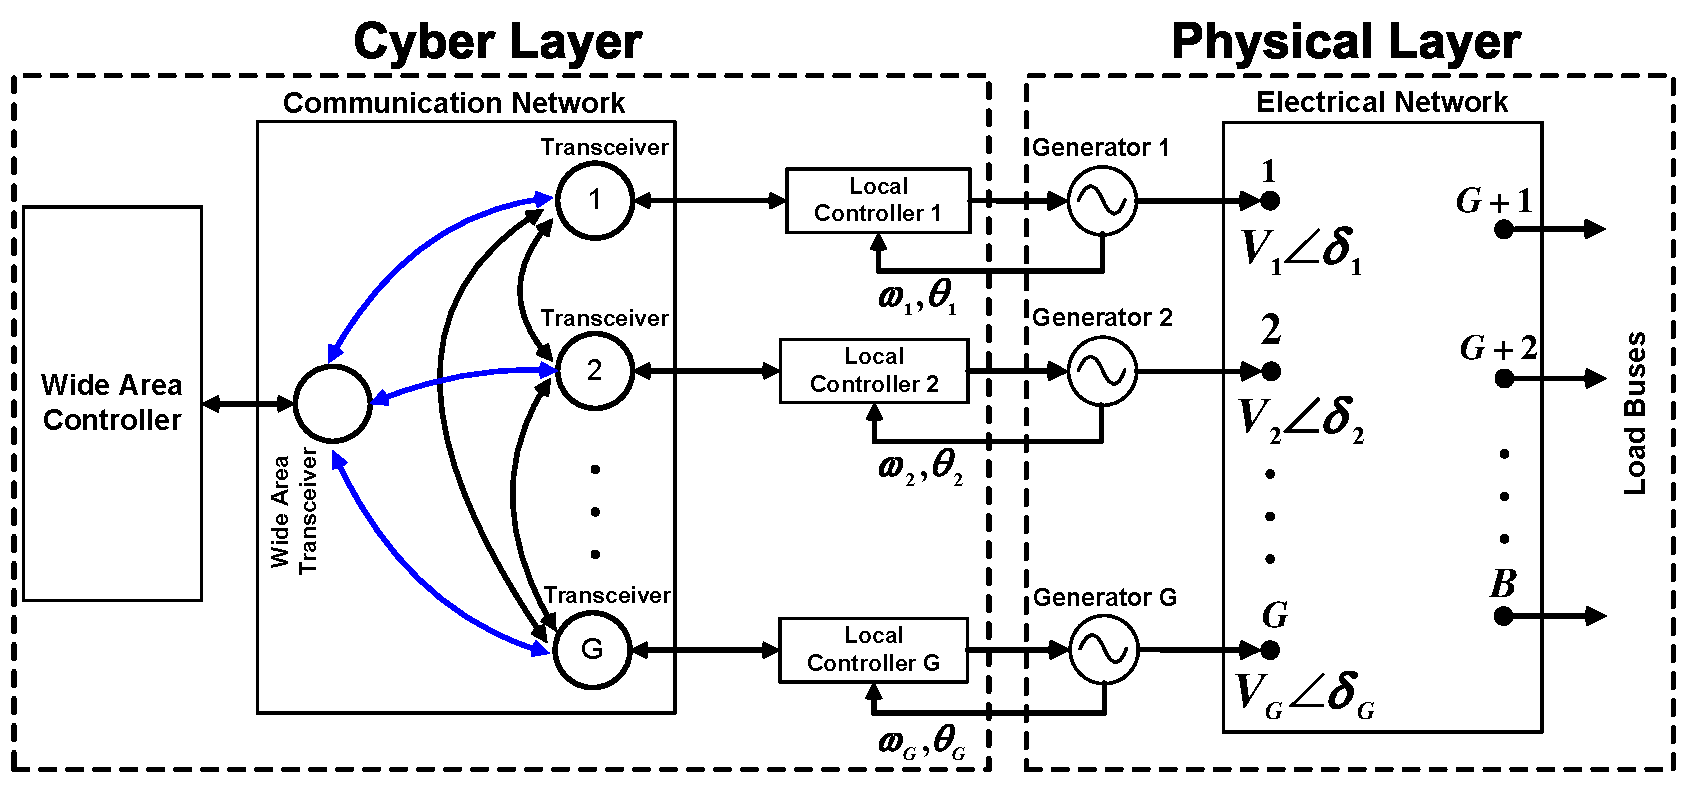
\includegraphics[width=6.5in]{chapters/se_nonlinear/figures/ps}\caption{A graphical depiction of the power system including both the physical and cyber layers.}\label{ps}
\end{center}
\end{figure*}



\subsection{Physical Layer Model}
Consider a power system comprising $G$ generators and $B$ buses. We assume that $G$ of the buses are generator buses, and that the remaining buses ($B-G$ buses) are load buses. Let $\mathcal{B}$ and $\mathcal{V}$ denote the set of buses and transmission lines, respectively. Here, we assume that the corresponding graph $\mathcal{H}(\mathcal{B},\mathcal{V})$ is connected, and that the network topology is fixed and known.

\textbf{Load buses:} Let $V_i$ and $\delta_i$ denote the magnitude and phase angle of the voltage phasor, respectively, at load bus $i\in\mathcal{L}$ where $\mathcal{L}$ is the set of load buses ($|\mathcal{L}|=B-G$). Let $P_i^e$ be the total active power leaving bus $i$ (i.e., the real power drawn by the load
at bus $i$ equals $-P_i^e$). $P_i^e$ can be computed by
\begin{align}
\label{load_bus}&P_i^e=\sum_{j\in\mathcal{B}}{{V_i V_j |y_{ij}|~\text{sin}(\delta_i-\delta_j+\phi_{ij})}}
\end{align}
where $y_{ij}=g_{ij}+\sqrt{-1} b_{ij}$ is the admittance of the line between buses $i$ and $j$, and $\phi_{ij}$ equals $\text{arctan}(g_{ij}/b_{ij})$. Note that $g_{ij}=g_{ji}\ge0$ and $b_{ij}=b_{ji}>0$ are the conductance and susceptance of the line between buses $i$ and $j$, respectively.




\textbf{Generator buses:} Let $\widehat{E_i}=E_i \phase{\theta_i}$ denote the internal voltage phasor of the generator connected to bus $i\in\mathcal{G}$ where $\mathcal{G}$ is the set of generator buses in the system. According to the synchronous machine theory, $E_i$ is constant and $\theta_i$ is the angular position of the generator rotor as measured with respect to a synchronous reference rotating at the nominal system electrical frequency $\omega_0$. We assume that the voltages at the generator buses are controlled via droop control, and that all the generator terminal buses are equipped with fast response energy storage units which are controlled via local and wide area controllers. Under these assumptions, for a synchronous generator connected to bus $i\in\mathcal{G}$, the dynamic variables are the generator phase angle $\theta_i$ and the rotor electrical angular speed $\omega_i$, and the generator dynamics can be described by \cite{Kundur}
\begin{align}
\label{swing1k}&\dot{\theta}_i=\omega_i-\omega_0\\
\label{swing2k}&\frac{2H_i}{\omega_0} \dot{\omega}_i=P_i^m-P_i^e-\textcolor{black}{\frac{d_i}{\omega_0} (\omega_i-\omega_0)}+ U_i
\end{align}
where $H_i$ is the machine inertia constant, $d_i$ is the damping coefficient of the generator, $U_i$ is the external stabilizing energy source at generator bus $i$, and $P_i^m$ is the mechanical power input to the generator. %Note that we have omitted the reactive
%power models for synchronous generators and loads as they are unnecessary for the analysis presented in this paper.


\textcolor{black}{Each generator terminal bus $i\in\mathcal{G}$ is equipped with a fast response energy storage, such as flywheels, to improve the system stability. Although synchronous generators are typically equipped with local controllers, such as exciter and governor controls, these local controllers only have access to local states and often have slow reaction to rapid system wide perturbations. A local cyber-enabled controller at the generator bus can potentially provide faster response time by using PMU
measurements of its neighbors \cite{facts_storage2}, \cite{facts_storage21}.}

The energy storage receives a measurement-based control signal computed from PMU measurements, and injects $U_i$ per unit values of power into bus $i$ if $U_i\ge0$; otherwise, it absorbs $U_i$ per unit values of power from bus $i$. Similar to the study in \cite{facts_storage2}, we develop a feedback linearization controller, and assume that the local controller at bus $i\in\mathcal{G}$ implements the following feedback linearization control law
\textcolor{black}{\begin{align}\label{Eq:Ui}
U_i = & - P^m_{i} + P_{i,\text{meas}}^e - F_i \left(\frac{\omega_i}{\omega_0} - 1 \right)
\end{align}}
where $P_{i,\text{meas}}^e$ is computed locally by the controller at bus $i$, and $F_i \geq 0$ is a design parameter. For more information on the impact of the parameter $F_i$ on the transient behavior of the system, we refer the reader to \cite{facts_storage2}, \cite{facts_storage21}.


\begin{figure}
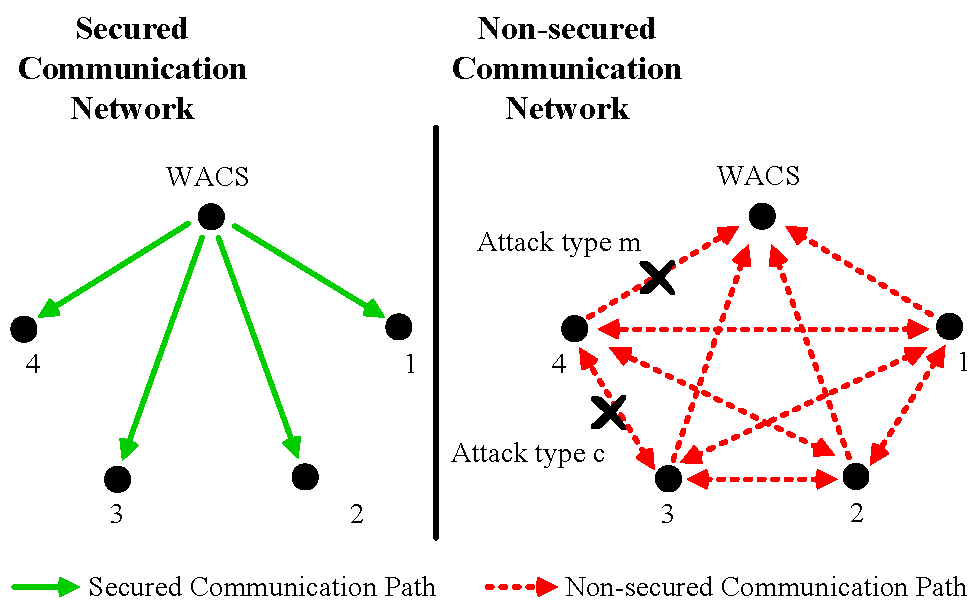
\includegraphics[width=0.42\textwidth]{chapters/se_nonlinear/figures/Comm_Net} \caption{A graphical depiction of the cyber network model: For simplicity, we focus on a system with only four generators in this figure. The graph in green (sold lines) shows the secured information flow (i.e., the set of information flows from the WACS to local controllers) while the graph in red (dotted lines) represents the set of non-secured information flows.}
\label{wacs}
\end{figure}

\subsection{Cyber Layer Model}
To maintain the system's stability, the system operator has equipped each generator with a local controller, PMU, and transceiver through which information can be exchanged with the local controllers of other generators as well as the WACS. These transceivers are connected through a communication network which sends PMU measurements, including rotors' speeds and generators' phase angles, to different transceivers. The communication network, PMUs, and transceivers are not secured, and hence they are subject to cyber attacks and communication failures.

In this study, we assume that the communication paths from the WACS to the local controllers are secured while other communication paths are not secured. Hence, the communication network interconnecting the transceivers can be described by two directed graphs, one for secured information flow and one for non-secured information flow, as shown in Fig.~\ref{wacs}.


\textcolor{blue}{Typically, the WACS is strongly protected against cyber attacks, and the local transceivers are more vulnerable to cyber attacks and communication failures than the WACS. For more information, we refer the reader to the North American Electric Reliability Corp. (NERC)s Critical Infrastructure Protection (CIP) standards \cite{nerc}. In particular, we refer the reader to 1) CIP-002 BES Cyber System Categorization that identifies control centers as a ``High Impact Rating", and 2) CIP-005 Electronic security Perimeter(s) and CIP-006 Physical Security of BES Cyber Systems to see what requirements are needed for high impact systems. The CIP Standards explain why we assume that the communication paths from the WACS to the local controllers is secured.}

%As mentioned earlier, in real power systems, measurements are telemetered from generating units to a wide area control system that performs secure state estimation and adjusts the set-point of each generator.
\textcolor{black}{To maintain the system's stability in the presence of attacks and failures, the WACS needs to perform secure state estimation before using the received data (e.g., $\omega_i$'s and $\theta_i$'s) for computing wide area control signals and for monitoring local controllers. To do so, we distinguish two types of attacks:
\begin{itemize}
\item \textbf{c-attack:} an attack that corrupts communication channels between local controllers.
\item \textbf{m-attack:} an attack that affects communication channels between a local controller and the WACS. %\textcolor{magenta}{ Is there any explanation/application such that we can justify $m$-attack? For example, any reviewers wonder why WACS $\rightarrow$ local controller is secured but local controller $\rightarrow$ WACS is non-secured.}
\end{itemize}
We assume that at any time instant, the cyber layer is subject to either a c-attack or an m-attack, but not both. This is discussed in detail in Section \ref{V_B}. However, both of these types of attacks and the set of attacked measurements can change at each time instant. These types of attacks are illustrated in Fig.~\ref{wacs} for a power system comprising four generators.}



\textcolor{black}{Next, by using the proposed secure state estimation technique, we develop a secure state estimator for estimating the dynamic states (i.e., generator' phase angles and rotors' speeds) of the power network.}


\section{Secure State Estimator for Wide Area \\Control Systems}\label{sec:application1}
The system dynamics and power flows can be described by the algebraic-differential equations in (\ref{load_bus})-(\ref{swing2k}). However, in order to use the proposed secure state estimation technique, we need to describe the system by a set of purely differential equations. To do so, we reduce the power network into a network of electro-mechanical oscillators, comprising the $G$ generators, by using the Kron reduction technique\footnote{\textcolor{black}{Kron reduction is a graph-based technique  used in power systems to eliminate algebraic load equations and to reduce the order of the interconnections between the synchronous generators \cite{kron}. This technique transforms an interconnected power system into an equivalent grid between the synchronous generators of the power system.}}. Let $\mathcal{V}^\prime$ denote the set of transmission lines between the $G$ generators after performing the Kron reduction technique, and let $\mathcal{K}(\mathcal{G},\mathcal{V}^\prime)$ denote the corresponding graph. This graph is connected and has $|\mathcal{V}^\prime|$ edges where $|\mathcal{V}^\prime| \le G (G-1)/2$.






We can now describe the power system by
\begin{equation}\label{eq:kron}
\begin{aligned}
\dot{\theta_i} & =\omega_i-\omega_0\\
\frac{2H_i}{\omega_0} \dot{\omega_i} &=P_i^m-\sum_{j\in\mathcal{N}_i}{{E_i E_j {|\widehat{y}_{ij}|} ~ \text{sin}(\theta_i-\theta_j+\widehat{\phi}_{ij})}}\\
&\quad-\textcolor{black}{\frac{d_i}{\omega_0} (\omega_i-\omega_0)}+ U_i
\end{aligned}
\end{equation}
where $\widehat{y}_{ij}=\widehat{g}_{ij}+\sqrt{-1} ~\widehat{b}_{ij}$ denotes the admittance of the Kron-reduced equivalent line between generators $i$ and $j$, and $\widehat{\phi}_{ij}$ equals $\text{arctan}(\widehat{g}_{ij}/\widehat{b}_{ij})$. $\mathcal{N}_i$ denotes the set of neighbors of generator $i$ in graph $\mathcal{K}(\mathcal{G},\mathcal{V}^\prime)$ (i.e., the reduced network).

In this study, we assume that the WACS performs a monitoring role and does secure estimation, and consider the mechanical input power $P_i^m$ and the storage control signal $U_i$ as local control signals which are computed based on PMU measurements and wide area control signals (e.g., area control error) \cite{Kundur}. When measurements are attacked, the estimated values of power flows or phase angles will not be equal to the actual values in the system (e.g., $P_{i,\text{meas}}^e \neq P_{i}^e$), and hence local controllers might send inaccurate signals to physical components. The WACS estimates attacks from measurements and communicates estimated attack signals to each generator. Then, each generator subtracts the estimated attack from the received measurements, as to obtain the most accurate values of $\omega_{i}$'s and $\theta_{i}$'s, and to make sure that the local controller will send accurate signals to the physical components that are under its control.




%%%%%%%%%%%%%%%%%%%%%%%%%%%%%%%%%
\vspace{-0.2cm}
\subsection{Formulation of Secure Estimation}

The local controller at generator $i$ computes the control input $U_i$ using (\ref{Eq:Ui}), in which $P_{i,\text{meas}}^e$ is calculated from PMU measurements:
\begin{equation}\label{eq:Pe_meas}
P_{i,\text{meas}}^e(t) = \sum_{j\in\mathcal{N}_i}{E_i E_j {|\widehat{y}_{ij}|} ~ \text{sin}\big(y^c_{ii}(t)-y^c_{ij}(t)+\widehat{\phi}_{ij}\big)},
\end{equation}
%In order to compute $P_{i,\text{meas}}^e$ and the local control signal $U_i$,
where $y^c_{ij}$ is the measured rotor angle of generator $j$ (i.e., $\theta_j$) received at generator $i$'s local controller. We assume that these PMU measurements are subject to attack:
\begin{equation}\label{Eq:yc}
\begin{aligned}
y^c_{ij}(t) & = \theta_j(t) + e^c_{ij} (t),~ i \in \mathcal{G},~j \in \mathcal{N}_i \cup \{i\}, \,
\end{aligned}
\end{equation}
where $e^c_{ij}$ represents the attack signal. As mentioned earlier, we refer to this as a c-attack (see Fig.~\ref{wacs}).
%Note that $e^c_{ji}$ represents the corruption in the measurement of $\theta_i$ received at generator $j$, thus $e^c_{ij}$ and $e^c_{ji}$ represent two distinct variables.
In addition, we assume $e^c_{ii}(t) = 0$ for all $t$. Note that $\theta_i$ is measured locally, and therefore it is not subject to cyber attack, i.e., $y^c_{ii}(t) = \theta_i(t)$ for all $t$.
%Finally, $P^m_i$ represents the input mechanical power to generator $i$, thus is known to generator $i$.

%To enable the WACS to perform secure estimation, each generator sends all of its measurements to the WACS. In other words, the WACS receives the following measurements
To performs secure estimation, the WACS receives measurements $y^m_{ij}$ from all the local controllers. Since we assume the communication flows from the local controllers to the WACS are not secured, measurements $y^m_{ij}$ can be subject to attack:
\begin{equation}\label{Eq:ym}
\begin{aligned}
y^m_{ij}(t) &= y^c_{ij}(t) + e^m_{ij}(t),~i \in \mathcal{G},~j \in \mathcal{N}_i \cup \{i\} \,
\end{aligned}
\end{equation}
where $e^m_{ij}$ represents the corruption in $y^c_{ij}$. We refer to these attacks as m-attacks (see Fig.~\ref{wacs}).

We now apply the forward Euler discretization scheme to this continuous-time system and obtain the following discrete-time approximation, assuming a constant discretization step $T_s$ for all $k$:
\begin{equation}
\begin{aligned}
\theta_i (k+1) &= \theta_i(k) + T_s \big(w_i(k) - \omega_0\big) \\
\omega_i(k+1)
	&= \alpha~\omega_i(k) + \beta \\
	& \quad + \sum_{j\in \mathcal{N}_i} f_{ij} \big(\theta_i(k), \theta_j(k), y^c_{ii}(k), y^c_{ij}(k)\big) \\
\end{aligned}
\end{equation}
where \textcolor{black}{$\alpha = 1- \frac{T_s (d_i + F_i)}{2H_i}$, $\beta = \frac{T_s  \omega_0(d_i+F_i)}{2H_i}$}, $f_{ij} (\cdot) = \tilde G_{ij} \big[ \sin \big(\theta_i(k) - \theta_j(k) + \widehat{\phi}_{ij}\big) - \sin \big(y^c_{ii}(k) - y^c_{ij}(k)+\widehat{\phi}_{ij}\big) \big] $
and $\tilde G_{ij} = - \frac{T_s \omega_0 E_i E_j |\widehat{y}_{ij}|}{2H_i}$.

Using (\ref{Eq:yc}) and (\ref{Eq:ym}), $f_{ij} (\cdot)$ can be re-written in terms of $y^m_{ij}$'s, which are the measurements received at the WACS, as follows:
\begin{equation} \label{Eq:case2_f_ij}
\begin{aligned}
	f_{ij} (\cdot ) &= \tilde G_{ij} \big[ \sin \big(\widehat{\phi}_{ij} + \theta_i(k) - \theta_j(k)\big) \\
		& \quad- \sin \big(\widehat{\phi}_{ij} + y^c_{ii}(k) - y^c_{ij}(k)\big) \big]\\
		& = \tilde G_{ij}  \sin \big(\widehat{\phi}_{ij} + y^m_{ii}(k) - y^m_{ij}(k) - e^m_{ii}(k) \\
		& \quad + e^m_{ij}(k) + e^c_{ij}(k)\big) - \tilde G_{ij} \sin \big(\widehat{\phi}_{ij} + y^m_{ii}(k) \\
		& \quad - y^m_{ij}(k) - e^m_{ii}(k) + e^m_{ij}(k)\big) \\
		& = G_{ij}^s (k) \epsilon_{ij}^c  (k)  -  G_{ij}^c  (k)  \epsilon_{ij}^s (k),
\end{aligned}\nonumber
\end{equation}
where $ G_{ij}^s(k) = \tilde G_{ij} \sin \big(\widehat{\phi}_{ij} + y^m_{ii}(k) - y^m_{ij}(k)\big)$, $ G_{ij}^c (k) = \tilde G_{ij} \cos \big(\widehat{\phi}_{ij} + y^m_{ii}(k) -y^m_{ij}(k)\big)$ are known to the WACS. On the other hand, $\epsilon_{ij}^c$ and $\epsilon_{ij}^s$ are functions of unknown attack signals and are defined as:
\begin{equation}\label{eq:epsilon_cs}
\begin{aligned}
\epsilon_{ij}^c(k) &= \cos \big(e^m_{ii}(k) - e^m_{ij}(k) - e^c_{ij}(k)\big) \\
& \quad - \cos \big(e^m_{ii}(k) - e^m_{ij}(k)\big) \\
\epsilon_{ij}^s (k) &= \sin \big(e^m_{ii}(k) - e^m_{ij}(k) - e^c_{ij}(k)\big) \\
& \quad - \sin \big(e^m_{ii}(k) - e^m_{ij}(k)\big).
\end{aligned}
\end{equation}
%In (\ref{Eq:case2_f_ij}), the second equality uses $\theta_{i}(k) = y^c_{ii}(k) = y^m_{ii}(k) - e^m_{ii}(k)$, $\theta_{j}(k) = y^c_{ij}(k) - e^c_{ij}(k) = y^m_{ij}(k) - e^m_{ij}(k) - e^c_{ij}(k)$.
In other words, $f_{ij}(\cdot)$ is now a linear function of the unknowns: $\epsilon_{ij}^c(k)$ and $\epsilon_{ij}^s(k)$, whose coefficients can be computed by the WACS from the received measurements. In addition, if there is no attack on any of the communication channels in the system at time slot $k$, then $\epsilon_{ij}^c (k) = \epsilon_{ij}^s (k) = 0$.

The state space model of the $i$-th generator is given by:
\begin{equation}
\begin{aligned}
x_i(k+1) &= A_i x_i(k) + q_i + H_i(k) \epsilon_i(k) \\
& = \begin{bmatrix} 1 & T_s \\ 0 & \alpha \end{bmatrix} x_i(k) + \begin{bmatrix} -T_s \omega_0 \\ \beta \end{bmatrix} + \begin{bmatrix} 0 \\ h_i(k)^\top \end{bmatrix} \epsilon_i(k)
%y_i(k) &= C_i x_i(k) \\
\end{aligned}
\end{equation}
where the state vector $ x_i(k) = \begin{bmatrix}  \theta_i(k), \omega_i(k) \end{bmatrix}^\top$ and
\begin{equation}
\begin{aligned}
h_i(k)^\top & = \big[ G_{i\mathcal{N}_i(1)}^s(k), \cdots, G_{i\mathcal{N}_i(l_i)}^s(k), \\
& \quad \quad \quad G_{i\mathcal{N}_i(1)}^c(k),  \cdots,  G_{i\mathcal{N}_i(l_i)}^c(k) \big] \in \mathbb{R}^{1 \times 2l_i}\\
\epsilon_i(k) & =  \big[\epsilon_{i\mathcal{N}_i(1)}^c(k), \cdots , \epsilon_{i\mathcal{N}_i(l_i)}^c(k), \\
& \quad\quad\quad \epsilon_{i\mathcal{N}_i(1)}^s (k), \cdots, \epsilon_{i\mathcal{N}_i(l_i)}^s (k) \big] ^\top \in \mathbb{R}^{2l_i \times 1}.
\end{aligned}\nonumber
\end{equation}
Here, $\mathcal{N}_i(j)$ is the $j$-th generator in the neighborhood of generator $i$ and $l_i$ is the cardinality of the set $\mathcal{N}_i$.
%$H_i(k) \triangleq \begin{bmatrix} 0_{1 \times 2l_i} \\ h_i(k)^\top \end{bmatrix} \in \mathbb{R}^{2 \times 2l_i}$, where $h_i(k)^\top = \begin{bmatrix} G_{i\mathcal{N}_i(1)}^s(k), \cdots, G_{i\mathcal{N}_i(l_i)}^s(k), G_{i\mathcal{N}_i(1)}^c(k),  \cdots,  G_{i\mathcal{N}_i(l_i)}^c(k) \end{bmatrix} \in \mathbb{R}^{1 \times 2l_i}$. Here $\mathcal{N}_i(j)$ presents the $j$-th node in the neighborhood of generator $i$ and $l_i$ represents the cardinality of the set $\mathcal{N}_i$.

Consider the enlarged system with $G$ generators in the network:
\begin{equation}\label{eq:state_space_N}
\begin{aligned}
X(k+1) & = AX(k) + q + H(k) \epsilon(k) \\
Y(k) & = CX(k) + DE(k)
\end{aligned}
\end{equation}
where
\begin{equation}
\begin{aligned}
X(k) &= \begin{bmatrix} x_1(k); \cdots; x_G(k) \end{bmatrix} \in \mathbb{R}^{2G\times 1} \\
A &= \text{blkdiag} \{ A_1, \cdots, A_G\} \in \mathbb{R}^{2G\times 2G}\\
q &= \begin{bmatrix} q_1; \cdots; q_G \end{bmatrix} \in \mathbb{R}^{2G\times 1}\\
H(k)& = \text{blkdiag} \{ H_1(k), \cdots, H_G(k) \}  \in \mathbb{R}^{2G\times 4L }\\
\epsilon(k) &\triangleq \begin{bmatrix} \epsilon_1(k); \cdots; \epsilon_G(k)\end{bmatrix} \in \mathbb{R}^{4L \times 1}  \\
Y(k) &= \begin{bmatrix} Y_{i}(k); \cdots; Y_G(k) \end{bmatrix} \in \mathbb{R}^{(G+2L) \times 1} \\
Y_i(k) & = \begin{bmatrix} y_{ii}(k); y_{i\mathcal{N}_i(1)}(k); \cdots; y_{i\mathcal{N}_i(l_i)}(k) \end{bmatrix} \in \mathbb{R}^{(1+l_i) \times 1} \\
%C &\triangleq \begin{bmatrix} C^1; \cdots; C^G\end{bmatrix}  \in \mathbb{R}^{(N+2L)\times 2N}\\
D &= \begin{bmatrix} D_1, D_2 \end{bmatrix}  \in \mathbb{R}^{(G+2L)\times (G+4L)}\\
%D_1 &\triangleq \text{blkdiag} \{d_1, \cdots, d_G\} \in \mathbb{R}^{(N+2L) \times 2L} \\
D_1 &= \text{blkdiag} \left \{ \begin{bmatrix} 0 \\ I_{l_1, l_1} \end{bmatrix}, \cdots, \begin{bmatrix} 0 \\ I_{l_G, l_G} \end{bmatrix} \right \} \in \mathbb{R}^{(G+2L) \times 2L} \\
D_2 & = I_{G+2L, G+2L} \in \mathbb{R}^{(G+2L) \times (G+2L)} \\
E(k) &=  \begin{bmatrix} E^c_1(k); \cdots; E^c_G(k); E^m_1(k) ; \cdots;  E^m_G(k) \end{bmatrix} \\
& \quad\in \mathbb{R}^{(G+4L) \times 1} \\
E^c_i(k) & = \begin{bmatrix} e^c_{i\mathcal{N}_i(1)}(k); \cdots; e^c_{i\mathcal{N}_i(l_i)}(k) \end{bmatrix} \in \mathbb{R}^{l_i \times 1} \\
E^m_i(k) & = \begin{bmatrix} e^m_{ii}; e^m_{i\mathcal{N}_i(1)}(k); \cdots; e^m_{i\mathcal{N}_i(l_i)}(k) \end{bmatrix} \in \mathbb{R}^{(1+l_i) \times 1}
\end{aligned}\nonumber
\end{equation}
and $L = \frac{\sum_i l_i}{2}$ represents the total number of edges / links in the network. Matrix $C \in \mathbb{R}^{(G+2L)\times 2G}$ is given as follows: let the $a$-th element of vector $Y$ be $y^m_{ij}$, then the $(a,b)$-th entry of $C$ is given by
\begin{equation}
C_{(a,b)} = \begin{cases}1 & \mbox{if } 2j-1 = b \\ 0 & \mbox{otherwise.} \end{cases} \nonumber
\end{equation}

\noindent
Consider $T$ time steps of measurements (i.e., $k = \{0, \cdots, T-1 \}$) and define:
\begin{equation}
\bar Y = \begin{bmatrix} Y (0)  \\ Y (1) - C q  \\ \vdots \\ Y(T-1) - C \sum_{m=0}^{T-2}A^{T-2-m} q \end{bmatrix} \in \mathbb{R}^{(G+2L)T \times 1}
\end{equation}
then
\begin{equation}\label{eq:Ebar_Psi}
\bar Y = \Phi X(0) + \Psi  \bar E
\end{equation}
where $\Phi = \begin{bmatrix} C; CA ; \cdots ; CA^{T-1} \end{bmatrix} \in \mathbb{R}^{(G+2L)T \times 2G}$ is \textcolor{black}{the $T$-step observability matrix of the system}, $\bar E = \begin{bmatrix} E(0); \cdots; E(T-1); \epsilon(0); \cdots; \epsilon(T-2) \end{bmatrix} \in \mathbb{R}^{((G+4L)T + 4L(T-1)) \times 1} $ and $\Psi = \begin{bmatrix} \Psi_{1} & \Psi_{2} \end{bmatrix}$, with $\Psi_{1} \in \mathbb{R}^{(G+2L)T \times (G+4L)T}$ and $\Psi_{2}\in \mathbb{R}^{(G+2L)T \times 4L(T-1)}$ as follows:
\begin{equation}
\begin{aligned}
\Psi_{1} &= \text{blkdiag} \{ D, \cdots, D \} \\
\Psi_{2} &= \begin{bmatrix}   0 &  0  &  \cdots    	\\
   			        C H(0) & 0 &  \cdots  	\\
			       CAH(0) &  CH(1) & \cdots	\\
			        \vdots & \vdots  &  \ddots \\
			       CA^{T-2}H(0) & \cdots & CH(T-2) \\			
			    \end{bmatrix}	.
\end{aligned}\nonumber
\end{equation}

\noindent
We can choose $\Omega \in \mathbb{R}^{ ((G+2L)T - 2G)\times (G+2L)T}$ such that $\Omega \Phi = 0$, then:
\begin{equation}\label{eq:Ebar_OmegaPsi}
	\tilde Y = \Omega \bar Y = \Omega \Psi \bar E,
\end{equation}
where $\Omega \Psi \in \mathbb{R}^{((G+2L)T - 2G) \times ((G+4L)T + 4L(T-1))}$.

%%%%%%%%%%%%%%%%%%%%%%%%%%%%%%

\subsection{Challenges in Secure Estimation due to the Power System's Dynamics}\label{V_B}
The linear system in (\ref{eq:Ebar_OmegaPsi}) is in the form of (\ref{eq:E_est}). Hence, from Lemma \ref{lem:CS}, $\bar E$ has a unique $s$-sparse solution if all subsets of $2s$ columns of  $\Omega\Psi$ are linearly independent.
We now explain that this is not the case in the power systems example as some columns of $\Psi$ are linearly dependent.
Let us begin with the following: consider a matrix-vector multiplication $M \cdot v$, where $M = [ m_1, \cdots, m_n ] \in \mathbb{R}^{l \times n}$ and $m_i$ is the $i$-th column of $M$, $v = [ v_1, \cdots, v_n ] ^\top \in \mathbb{R}^{n \times 1}$, and $v_i$ is the $i$-th entry of $v$. In the sequel, the phrase ``the column of $M$ that corresponds to $v_i$" refers to the column of $M$ that multiplies the $v_i$ entry in the matrix-vector multiplication, i.e., $m_i$.

We now explain why $\Psi_2$ is rank deficient.
Observe that for all $i$ and $k$, the first row of $H_i(k)$ is equal to zero. Therefore given any matrix $M = \begin{bmatrix} m_1 & m_2 \end{bmatrix} \in \mathbb{R}^{l \times 2}$, where $m_1$ and $m_2$ are the columns of $M$, we have:
\textcolor{black}{\begin{align}
\operatorname{rank} \big( M \cdot H_i(k) \big) &=  \operatorname{rank} \left( \begin{bmatrix} m_1 & m_2  \end{bmatrix} \cdot \begin{bmatrix} 0 & 0 & \cdots \\ h_{21} & h_{22} & \cdots \end{bmatrix} \right)\nonumber\\
	= &\operatorname{rank} \left( \begin{bmatrix} h_{21} m_2 & h_{22} m_2 & \cdots \end{bmatrix} \right)=1.
\end{align}}
Since $H(k)$ is block diagonal, we can show that $\Psi_2$ is also rank deficient.
%To see this more clearly, the first row of $H_i(k)$ are zeros, therefore given any matrix $M$, $\text{rank}(MH_i(k)) = 1$. In other words, all columns of $\Psi_2$ that correspond to the same $H_i(k)$ are linearly dependent. In (\ref{eq:Ebar_OmegaPsi}), $\Psi_2$ multiplies the $\epsilon(k)$ terms in $\bar E$, consequently, the $\epsilon(k)$'s may not be identifiable.
Next, from (\ref{Eq:yc}) and (\ref{Eq:ym}), we have $y^m_{ij}(k) = \theta_j(k) + e^c_{ij}(k) + e^m_{ij}(k)$, which means for a given ($i,j$)-pair ($i \neq j$) and a given time slot $k$, the two columns of $\Psi_1$ that correspond to the two terms $e^c_{ij}(k)$ and $e^m_{ij}(k)$ in $\bar E$ are identical, i.e., linearly dependent. Therefore, by Lemma \ref{lem:CS}, the solution $\bar E$ obtained by solving (\ref{eq:Ebar_OmegaPsi}) (i.e., the estimation algorithm introduced in Section \ref{sec:review}) is not unique.
Does this mean we can not uniquely recover the attack signal?
A closer analysis reveals the specific entries in $\bar E$ that cannot be uniquely identified, and shines light on how to overcome this challenge. Our observations are as follows:
\begin{enumerate}
\item Observe from (\ref{eq:Ebar_OmegaPsi}) that $\Psi_2$ multiplies the $\epsilon(k)$ terms in $\bar E$, i.e., $\big( \epsilon(0), \cdots, \epsilon(T-2) \big)$.
Linear dependence of the columns of $\Psi_2$ causes the $\epsilon(k)$ terms to be unidentifiable.
However, $\epsilon (k)$ can be computed from $E(k)$ using (\ref{eq:epsilon_cs}). In other words, although the $\epsilon(k)$ terms in the solution $\bar E$ are not unique, as long as the $E(k)$ terms in $\bar E$ are unique, then we can determine the $\epsilon (k)$ terms uniquely using (\ref{eq:epsilon_cs}).

\item The identical columns of $\Psi_1$ that correspond to the two terms $e^c_{ij}(k)$ and $e^m_{ij}(k)$ in $\bar E$ means that it is only possible to uniquely identify the sum $e^c_{ij}(k)+e^m_{ij}(k)$, but not the individual terms: $e^c_{ij}(k)$ and $e^m_{ij}(k)$. To overcome this challenge, we make the assumption that at any time $k$, the system is subject to either a c-attack or an m-attack, but not both. In other words, $e^m_{ij}(k)$ and $e^c_{ij}(k)$ cannot both be non-zero, thus making them identifiable.
\end{enumerate}
Next, we explain our secure estimation algorithm.

%%%%%%%%%%%%%%%%%%%%%%%%%%%%%%%

\subsection{Assumptions and Secure Estimation with 2-Step Delay}


As mentioned earlier, we assume that at any time slot $k$, the cyber layer is subject to either a c-attack or an m-attack, but not both at the same time.
However, both the types of attacks and the set of attacked measurements can change at each time step. In addition, the WACS does not know \textit{a priori} which type of attack the network is subjected to. Hence, secure estimation techniques are required to determine the type of attack, as well as the exact corruption signals.

Using the difference equation in (\ref{eq:state_space_N}), we find that
\textcolor{black}{
\begin{align}\label{eq:2step_delay}
&f_\text{2-step}\big (\epsilon(k-2), E(k) \big)  = Y(k) - CA^2\cdot X(k-2) - CAq  \nonumber\\
	&   - Cq - CA\cdot H(k-2)\cdot \epsilon(k-2)  - DE(k)= 0
\end{align}}
where the first equality uses $CH(k)=0$ for all $k$. Observe that if it is an m-attack at time $k$, then $e^c_{ij}(k) = 0$ and $e^c_{ij}(k) + e^m_{ij}(k) = e^m_{ij}(k)$, furthermore, $\epsilon(k) = 0$. On the other hand, if it is a c-attack at time $k$, then $e^m_{ij}(k) = 0$ and $e^c_{ij}(k) + e^m_{ij}(k) = e^c_{ij}(k)$, in addition, $\epsilon(k) \neq 0$.
Combining these two observations with (\ref{eq:2step_delay}), we propose the following algorithm which can be used by the WACS to determine the type of attack and the exact corruption signals, with a 2-step delay.

We first introduce some notation used in the algorithm. Let $E_\text{b}(k)$ denote the estimated vector $E(k)$ without imposing the assumption that only a c-attack or an m-attack can occur.  $E_{\text{c-att}}(k)$ and $E_{\text{m-att}}(k)$ denote the estimated vector $E(k)$ if it is a c-attack or an m-attack at time $k$, respectively, and can be computed from $E_\text{b}(k)$. For example, to obtain $E_{\text{c-att}}(k)$, we set all $e^m_{ij}$ terms in $E_{\text{c-att}}(k)$ to zero, and set all $e^c_{ij}$ terms equal to the sum of corresponding $e^c_{ij}$ and $e^m_{ij}$ terms in $E_\text{b}(k)$. We can obtain $E_{\text{m-att}}(k)$ in a similar fashion. Finally, $\epsilon_{\text{c-att}}(k)$ and $\epsilon_{\text{m-att}}(k)$ are the $\epsilon(k)$ vectors computed from $E_{\text{c-att}}(k)$ and $E_{\text{m-att}}(k)$, respectively.
With these notations in hand, we now present our estimation algorithm in Algorithm \ref{al:se}.


\begin{algorithm}
\caption{Secure Estimation}
\label{al:se}
\begin{algorithmic}[1]
%\State Initialize the KF
\For{each $k$}
	\State Estimate $\bar E(k)$ by solving the following $l_1$-minimization problem:
		\begin{equation}
		\bar E_\text{b}(k) = \arg \min \| \bar E \|_{l_1} ~\text{subject to}~ \tilde Y = \Omega\Psi \bar E.
		\nonumber
		\end{equation}
	\State Extract $E_\text{b}(k-2)$ and $E_\text{b}(k)$ from $\bar E_\text{b}(k)$.
	\State Evaluate equation (\ref{eq:2step_delay}) for the case with an m-attack at time $k-2$, using the observation that $\epsilon_\text{m-att}(k-2) = 0$.
	\State Evaluate equation (\ref{eq:2step_delay}) for the case with a c-attack at time $k-2$, by first computing $E_\text{c-att}(k-2)$ and then use (\ref{eq:epsilon_cs}) to obtain $\epsilon_\text{c-att}(k-2)$.
	\If{$\|f_\text{2-step}\big (\epsilon_\text{c-att}(k-2), E_\text{b}(k) \big) \| < \|f_\text{2-step}\big (\epsilon_\text{m-att}(k-2), E_\text{b}(k) \big) \|$}
		\State It is a c-attack at $k-2$: $E(k-2) = E_\text{c-att}(k-2)$ and $\epsilon(k-2) = \epsilon_\text{c-att}(k-2)$
	\Else
		\State It is an m-attack at $k-2$: $E(k-2) = E_\text{m-att}(k-2)$ and $\epsilon(k-2) = \epsilon_\text{m-att}(k-2)= 0$
	\EndIf
\EndFor
\end{algorithmic}
\end{algorithm}



To summarize, as a result of the system dynamics and the proposed model, it is not possible to recover the exact corruption if the system is subjected to both c- and m-attacks at the same time. In light of this, we make the simplifying assumption that at any time $k$, the system may only be subject to one type of attack. However, the type of attack can change over time. Then, by comparing the actual measurements with the system trajectories that would result from each type of attack, we can determine both the attack type and the exact corruption signals, with a 2-step delay. Note that at time $k$, this secure state estimation algorithm is able to detect the presence of attacks at times $k-1$ and $k$, merely not the exact attack signals.
Next, we numerically demonstrate the effectiveness of the proposed state estimation algorithm.





% !TEX root = ../../thesis.tex

\section{Numerical Example}\label{sec:example}
We focus on the New England power system comprising 10 generators and 39 buses, and simulate the system for $t=20$ seconds \textcolor{black}{with a discretization step of $1/60$ seconds}. The values of the system parameters are taken from \cite{new_england1}, \cite{new_england2}. The power system is running under normal condition from $t=0$ to $t=2$ seconds. \textcolor{black}{At $t=2$ seconds, a three-phase fault occurs at Bus 17. Then, Line 17�-18 is tripped out to clear the fault. However, the WACS is unaware of this fault at this time. Two seconds later, at $t=4$ seconds, the WACS detects the occurrence of this fault, i.e., there is a $2$~second-delay in the WACS being able to respond to the fault.} We conduct load flow analysis of the power system before and after the occurrence of the 3-phase fault, to find the values of $P_{i}^e$, $ \theta_i$, and $|E_i|$ for each generator. We demonstrate the effectiveness of our proposed secure estimation method through simulations of 3 different scenarios:
%\textcolor{black}{Do we have to explain what Line 17--18 is or is it obvious?}\textcolor{black}{I think it is clear that we are focusing on the New England system.}
\begin{enumerate}
\item \textit{Scenario 1:} There is no simultaneous cyber attack on the power system.
\item \textit{Scenario 2:} The power system is also under cyber attack, and it is not protected by secure estimation.
\item \textit{Scenario 3:} The power system is also under cyber attack, and it is protected by secure estimation.
\end{enumerate}

The plots titled ``No Attack'' in Figure~\ref{fig:SE} show the simulation results of Scenario 1: an attack-free power system under a three-phase fault. For clarity, only phase angles and rotor speeds of generators 1, 2 and 3 are shown in Figure~\ref{fig:SE}. At $t=0$ seconds, the system is under equilibrium, all ten generators' rotor speeds are at the nominal value, $\omega_0$, of 60~Hz, and their phase angles are $6.85^\circ$, $5.09^\circ$, $6.28^\circ$, $8.81^\circ$, $7.38^\circ,$ $11.30^\circ$, $14.74^\circ$, $8.35^\circ$, $7.63^\circ$ and $-13.11^\circ$, respectively. At $t=2$ seconds, a three-phase fault occurs at Bus 17 which causes a change in the line admittances ($y_{ij}$'s and $\phi_{ij}$'s) and consequently, the total active power leaving bus $i$, $P^e_i$. However, the WACS is unaware of this fault until $t=4$ seconds. \textcolor{black}{During this 2~second-delay, the WACS is unaware of the fault and continues to use the pre-fault line admittance values in the secure estimation algorithm. The local controllers at the generators continue to compute the control input $U_i$ using the received measurements from the WACS, which leads to a mismatch between $P^e_{i,\text{meas}}$ and $P^e_i$, and causes the phase angles and rotor speeds of the generators to deviate from their equilibrium. At $t=4$ seconds, the WACS becomes aware of the fault. It computes the new line admittance values under this fault, and uses the new line admittance values in the secure estimation algorithm. The local controllers then use the received estimates to compute the local control input $U_i$, making $P^e_{i,\text{meas}} = P^e_i$ again.} As a result, the generators' rotor speeds slowly converge back to 60~Hz and their rotor angles settle at new equilibrium values.



In Scenarios 2 and 3, in addition to the 3-phase fault, the power system is also subject to the following cyber attack. Malicious attacks targeted at generator 1 are injected from $t = 0.33$~seconds onwards. A set of 10 measurements that varies with time are corrupted. More specifically, at each time step, the attacker randomly chooses to perform either a c-attack or an m-attack.
In the case of a c-attack, the attacker corrupts phase angle measurements that generator 1 receives from all its 9 neighbors (i.e., $y^c_{1,2}, y^c_{1,3}, \ldots, y^c_{1,10}$) with independent Gaussian signals from the distribution $\mathcal{N} (0, 180^\circ)$. In addition, a constant signal of $90^\circ$ is injected into the measurement $y^c_{1,2}$.
In the case of an m-attack, the attacker randomly chooses 9 measurements from the set of 10 measurements that generator 1 submits to the WACS $(i.e., y^m_{1,1}, y^m_{1,2}, \ldots, y^m_{1,10})$, and corrupts each chosen measurement with an independent Gaussian signal from $\mathcal{N} (0, 180^\circ)$. Similarly, an additional constant signal of $90^\circ$ is injected into the measurement $y^m_{1,2}$.
%\textcolor{black}{Do we need the constant attack? It would be better to put an explanation.}
The left plot in Figure~\ref{fig:attack} shows the true attack signals. Rows 1 to 9 correspond to c-attacks: $e^c_{1,2}, e^c_{1,3}, \ldots, e^c_{1,10}$, and rows 10 to 19 correspond to m-attacks: $e^m_{1,1}, e^m_{1,2}, \ldots, e^m_{1,10}$. Since constant signals of $90^\circ$ are injected on top of the Gaussian attacks to $y^c_{1,2}$ or $y^m_{1,2}$ for c-attacks or m-attacks, respectively, the mean attack signals are higher for row 1 (i.e., $e^c_{1,2}$) and row 11 (i.e., $e^m_{1,2}$). For clarity, the measurements that are not attacked during the simulation are not shown.


In Scenario 2, no secure estimation-based protection is implemented. Therefore, when the system is under cyber attack, the local controller at generator 1 computes $P^e_{1,\text{meas}}$ using corrupted measurements, causing $P^e_{1,\text{meas}} \neq P^e_1$.
As a result, the feedback control law in (\ref{Eq:Ui}) fails to linearize the system dynamics (\ref{swing2k}).
The constant signal of $90^{\circ}$ injected on top of the Gaussian attacks causes oscillations in the rotor speed of generator 1 due to the sine term in its dynamics (refer to Equation~(\ref{Eq:Ui}) to (\ref{Eq:yc})). The oscillations in the rotor speed then leads to oscillations in generator 1's rotor angle.
The plots titled ``Under Attack, no SE'' in Figure~\ref{fig:SE} show that these oscillations are observed on top of the system's response to the 3-phase fault, and prevents generator 1's phase angle to reach a new equilibrium even after the fault has cleared.
In addition, the cyber attack causes larger differences in other generators' equilibrium rotor angles before and after the fault. For example, in Scenario 1, when there is no cyber attack, generator 2 and 3's rotor angles after the fault are $-14^{\circ}$ and $-8^{\circ}$ respectively. On the other hand, in Scenario 2, their post-fault equilibrium rotor angles are $-25^{\circ}$ and $-17^{\circ}$ respectively.


%This causes generator 1's rotor speed to deviate from the nominal value, which in turn, causes the generator's rotor angle to rapidly diverge from its equilibrium value, reaching $159^\circ$ within 7.3~sec, as shown in the left plots in Figure \ref{fig:SE}. When the phase angle difference between two generators exceeds $90^\circ$, the generators can potentially loose synchrony and trip. In this simulation, the phase angle difference between generators 1 and 10 exceeds $90^\circ$ at 4.78~sec.
%As shown in Figure \ref{fig:attack}, the proposed state estimation enables the WACS to reconstruct the rotor angles and rotational speeds of the generators accurately, and to prevent all possible failures.





\begin{figure}
\centering
%\vspace*{-0.3cm}
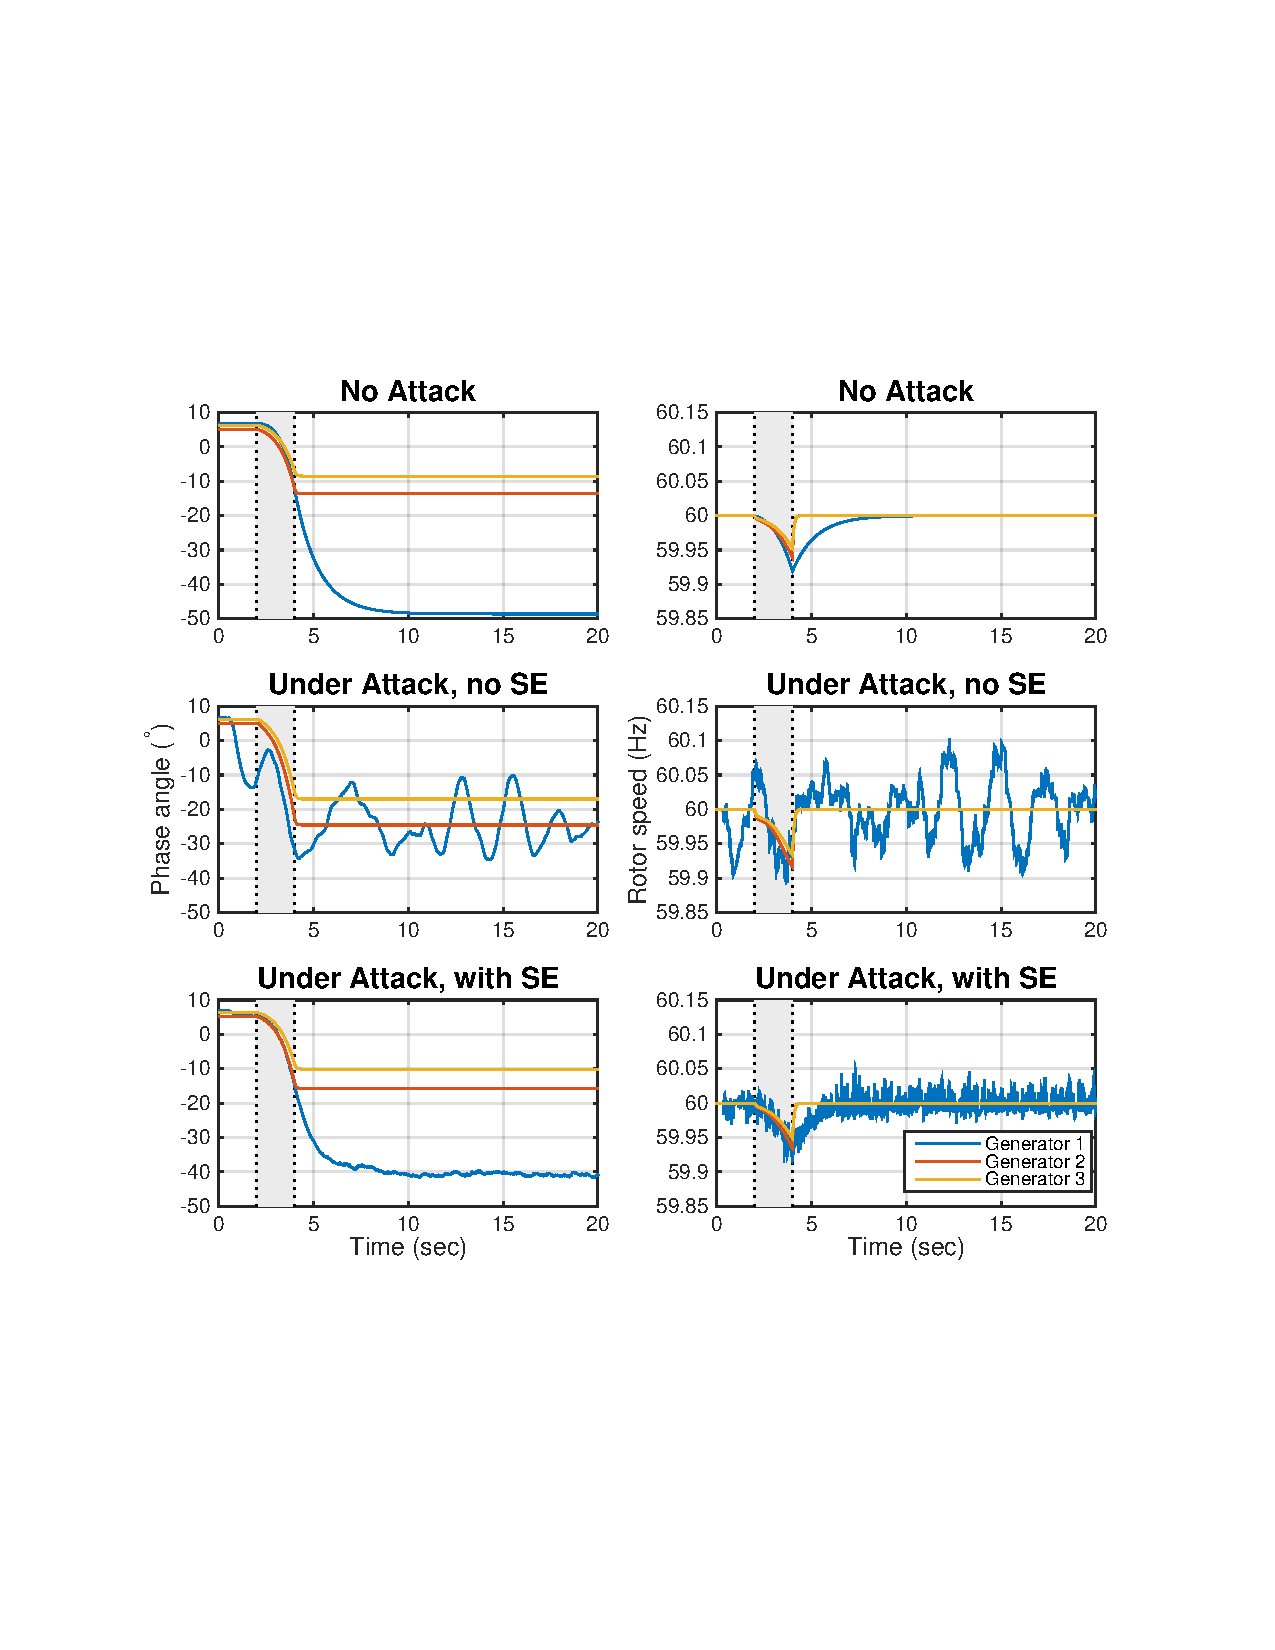
\includegraphics[scale=0.8]{chapters/se_nonlinear/figures/SE3.pdf}
%\vspace*{-0.8cm}
\caption{Evolution of phase angles and rotor speeds of generators 1, 2 and 3 under a 3-phase fault, in three scenarios: (1) there is no attack, (2) system is under attack and there is no secure estimation (SE), (3) system is under attack and WACS uses SE. Fault happens at $t=2$ seconds. Grey region marks the 2 seconds delay in WACS being informed of the fault. In (2), cyber attack causes generator 1's rotor angle and speed to oscillate. In (3), incorporating SE damps the large oscillations and makes the system's response more closely resemble that of (1).}
\label{fig:SE}
\end{figure}

\begin{figure}
\centering
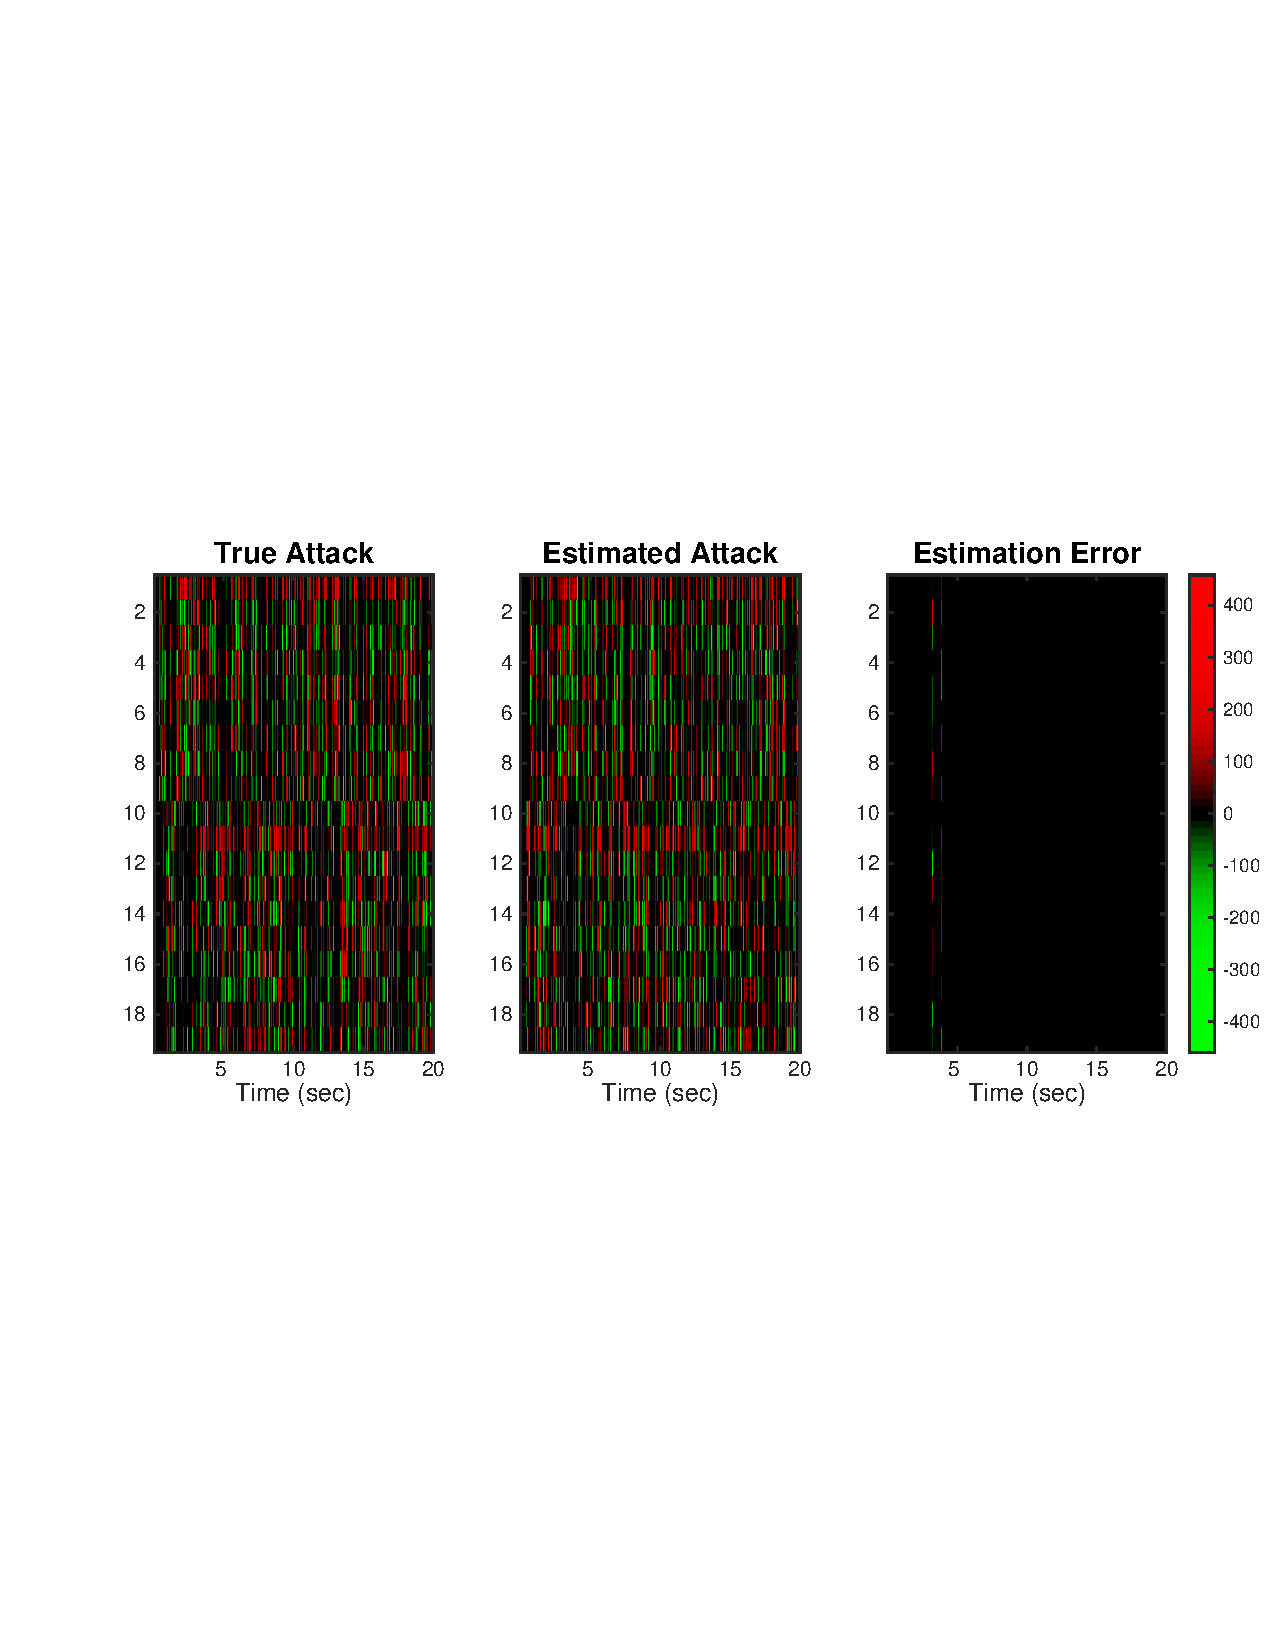
\includegraphics[scale=0.7]{chapters/se_nonlinear/figures/attack.pdf}
%\vspace*{-0.5cm}
\caption{True and estimated attack signals: The rows and columns correspond to attacked measurements and time steps, respectively. In subfigures ``True Attack'' and ``Estimated Attack'', the color indicates the attack signal: red is a positive attack, green a negative attack, and black is no attack. In subfigure ``Estimation Error'', the black color indicates there is zero estimation error for all measurements at all times.}
%\vspace*{-0.3cm}
\label{fig:attack}
\end{figure}


Finally, in Scenario 3, the power system is subject to the same cyber attack as in Scenario 2. However, the WACS uses secure estimation to protect the system against such attacks.
The center and right plots in Figure~\ref{fig:attack} show the secure estimator's estimated attack signal and the estimation error respectively.
The results show that the secure estimator correctly estimates the attack signal before the fault happens at $t=2$ seconds. Between $t=2$ and $t=4$ seconds, there are small estimation errors due to model mismatch as the WACS is unaware of the fault and continues to use the pre-fault line admittance values in the secure estimation algorithm. However, once the WACS is informed of the fault at $t=4$ seconds, the model mismatch is removed and estimation error is cleared. The estimated the attack signals are then subtracted from the corrupted measurements to recover the true rotor angles and speeds. The reconstructed measurements are communicated to all generators, and used to compute $P^e_{1,\text{meas}}$. By doing this, the local controllers obtain a value of $P^e_{1,\text{meas}}$ that is a more accurate estimate of the true $P^e_1$ than when no secure estimation was used.
The bottom plots, titled ``Under Attack, with SE'', in Figure~\ref{fig:SE} show the rotor angles and speeds of generators 1, 2, and 3 in this scenario.
Observe that throughout the simulation, generator 1's rotor angle is much more stable in this scenario than in Scenario 2.
In addition, note that when the power system is under cyber attack, the behavior of the system with secure estimation (Scenario 3) resembles more closely the system's behavior when there is no cyber attack (Scenario 1), than the system without secure estimation (Scenario 2) does.


As mentioned earlier, there is a 2-step estimation delay in the proposed secure state estimator. Our numerical results show that this estimation delay will not affect the phase angle and rotor speeds significantly. This can be explained by the fact that the attack signals effect on the system dynamics are scaled
by the matrix $H$ (see Equations (26) and (27)) whose entries are very small due to the small discretization time step (1/60 seconds) and the large generators' inertia (i.e., attack signals cannot immediately have a significant effect on the generators' phase angles and speeds).
\textcolor{black}{The simulation was repeated using a larger discretization time step of 1/30 seconds and the same observations were made (the control feedback gain $F_i$ was adjusted accordingly). Due to space limitations, we do not show the results here.}





\section{Conclusion}
\textcolor{black}{We propose a secure state estimator for two classes of nonlinear dynamical systems. We then focus on the wide area control of power systems, and develop an estimator for dynamic states in power systems under cyber-physical attacks and communication failures. Finally, we numerically show that the performance of the cyber layer in power systems can be significantly improved by using our estimator.} \textcolor{black}{One possible direction for future research is reducing the computational complexity of the secure state estimators. Note that the computational complexity increases with the time index. Therefore, computing an exact solution to the $l_1$-minimization problem in a recursive way can significantly reduce the time required to obtain a new estimate.}


%
%\begin{thebibliography}{00}
%
%\bibitem{cps1} F. Pasqualetti, F. Dorfler, and F. Bullo, ``Control-Theoretic Methods for Cyber-physical Security: Geometric Principles for Optimal Cross-Layer Resilient Control Systems," {\em in IEEE Control Systems}, vol. 35, no. 1, pp. 110--127, Feb. 2015.
%
%
%\bibitem{security_0} S. Sridhar, A. Hahn, and M. Govindarasu, ``Cyber-Physical System Security for the Electric Power Grid," {\em in Proceedings of the IEEE}, vol. 100, no. 1, pp. 210--224, Jan. 2012
%
%\bibitem{comm_net_1} X. Wang and P. Yi, ``Security framework for wireless communications
%in smart distribution grid," {\em IEEE Trans. on Smart Grid}, vol. 2, no. 4, pp. 809--818, Dec. 2011.
%
%\bibitem{comm_net_2} Y. Zhang, L. Wang, W. Sun, R. Green, and M. Alam, ``Distributed intrusion
%detection system in a multi-layer network architecture of smart
%grids," {\em IEEE Trans. on Smart Grid}, vol. 2, no. 4, pp. 796--808, Dec. 2011.
%
%\bibitem{comm_net_3} H. Li, L. Lai, and W. Zhang, ``Communication requirement for reliable
%and secure state estimation and control in smart grid," {\em IEEE Trans. on Smart
%Grid}, vol. 2, no. 3, pp. 476--486, Sep. 2011.
%
%\bibitem{comm_net_4} Q. Li and G. Cao, ``Multicast authentication in the smart grid with onetime
%signature," {\em IEEE Trans. on Smart Grid}, vol. 2, no. 4, pp. 686--696,
%Dec. 2011.
%
%\bibitem{comm_early_1} C. Alcaraz, C. Fernandez-Gago, and J. Lopez, ``An early warning system based on reputation for energy control systems," {\em IEEE Trans. on Smart Grid},
%vol. 2, no. 4, pp. 827--834, Dec. 2011.
%
%\bibitem{comm_early_2} C. W. Ten, J. Hong, and C. C. Liu, ``Anomaly detection for cybersecurity
%of the substations," {\em IEEE Trans. on Smart Grid}, vol. 2, no. 4, pp. 865--873,
%Dec. 2011.
%
%
%\bibitem{ctrl_sec8} H. Fawzi, P. Tabuada, and S. Diggavi, ``Secure estimation and control for
%cyber-physical systems under adversarial attacks," {\em IEEE Trans. on Automatic Control}, vol. 59, no. 6, pp. 1454--1467, June 2014.
%
%
%\bibitem{new2} Y. Shoukry and P. Tabuada, ``Event-Triggered State Observers for Sparse Sensor Noise/Attacks," {\em IEEE Trans. on Automatic Control}, no. 99, pp. 1--13, 2015.
%
%
%\bibitem{new3} S. Mishra, N. Karamchandani, P. Tabuada, and S. Diggavi, ``Secure state estimation and control using multiple (insecure) observers," {\em 53rd IEEE Conference on Decision and Control}, pp. 1620--1625, 2014.
%
%
%
%\bibitem{new4} M. S. Chong, M. Wakaiki, and J. P. Hespanha, ``Observability of linear systems under adversarial attacks," {\em in American Control Conference}, pp. 2439--2444, 2015.
%
%\bibitem{ctrl_sec9}  Q. Hu, Y. H. Chang,  and C. J. Tomlin, ``Secure Estimation for Unmanned Aerial Vehicles (UAVs) against Adversarial Attacks" International Council of the Aeronautical Sciences (ICAS), 2016.
%%%%%%%%%%%%%%%%%%%%%%%%%%%%%%%%%%%%%%%%%%%%%%%%%%%%%%%%%%%%%%%%%%%%%%%%%%%%%%%%%%%%%%%%%%%%
%\bibitem{new5} Y. Shoukry, P. Nuzzo, A. Puggelli, A. L. Sangiovanni-Vincentelli, S. A.
%Seshia, and P. Tabuada, ``Secure state estimation for cyber physical
%systems under sensor attacks: a satisfiability modulo theory approach,"
%arXiv pre-print, Dec. 2014.
%
%
%\bibitem{new6} M. Pajic, J. Weimer, N. Bezzo, P. Tabuada, O. Sokolsky, I. Lee,
%and G. Pappas, ``Robustness of attack-resilient state estimators," {\em in
%ACM/IEEE International Conference on Cyber-Physical Systems (ICCPS)}, 2014.
%
%\bibitem{new7} Y. Mo and B. Sinopoli, ``Secure control against replay attacks," {\em in
%Allerton Conference on Communication, Control, and Computing}, 2009.
%
%\bibitem{new8} C.-Z. Bai and V. Gupta, ``On Kalman filtering in the presence of a
%compromised sensor: fundamental performance bounds," {\em in American
%Control Conference (ACC)}, 2014.
%
%\bibitem{new9} J. Mattingley and S. Boyd, ``Real-time convex optimization in signal
%processing," {\em IEEE Signal Processing Magazine}, vol. 27, no. 3, pp. 50�-61, May 2010.
%
%\bibitem{new10} S. Farahmand, G. B. Giannakis, and D. Angelosante, ``Doubly robust
%smoothing of dynamical processes via outlier sparsity constraints," {\em IEEE
%Trans. on Signal Processing}, vol. 59, no. 10, pp. 4529-�4543, Oct. 2011.
%
%\bibitem{Kundur} P. Kundur, \emph{Power System Stability and Control}. McGraw-Hill, 1994.
%
%\bibitem{nonlin_est} S. Wang, W. Gao, and A. P. S. Meliopoulos, ``An alternative method for power system dynamic state estimation based on unscented transform,"
%{\em IEEE Trans. on Power Systems}, vol. 27, no. 2, pp. 942--950, May 2012.
%
%\bibitem{kundur_time} S. Liu, B. Chen, T. Zourntos, D. Kundur, and K. Butler-Purry, ``A Coordinated Multi-Switch Attack for Cascading Failures in Smart Grid," {\em IEEE Trans. on Smart Grid}, vol. 5, no. 3, pp. 1183--1195, May 2014.
%
%
%\bibitem{shoukry} Y. Shoukry, P. Nuzzo, N. Bezzo, A. L. Sangiovanni-Vincentelli, S. A. Seshia, and P. Tabuada, ``A satisfiability modulo theory approach to secure state reconstruction in differentially flat systems under sensor attacks,'' {\em arXiv:1509.03262v1}, Sep. 2015.
%
%%%%%%%%%%%%%%%%%%%%%%%%%%%%%%%%%%%%%%%%%%%%%%%%%%%%%%%%%%%%%%%%%%%%%%%%%%%%%%%%%%%%%%%%%%%%
%
%
%
%
%\bibitem{pmu_w_0} A. Chakrabortty and P. Khargonekar, ``Introduction to Wide-Area Control of Power Systems," {\em in Proc. of American Control Conference}, pp. 6758–-6770, 2013.
%
%
%\bibitem{pmu_w_1} Y. Liu \textit{et al.}, ``A US-wide power systems frequency monitoring network,"
%{\em in Proc. IEEE PES General Meeting}, pp. 1914--1921, Jun. 2006.
%
%
%\bibitem{pmu_w_3} A. R. Messina, V. Vittal, D. Ruiz-Vega, and G. Enriquez-Harper,
%``Interpretation and visualization of wide-area PMU measurements
%using Hilbert analysis," {\em IEEE Trans. on Power Systems}, vol. 21, no. 4, pp.
%1760--1771, 2006.
%
%\bibitem{wacs_ref8} M. R. Younis, and R. Iravani, ``Wide-area damping control for inter-area oscillations: A comprehensive review," {\em Electrical Power \& Energy Conference (EPEC)}, pp. 1--6, Aug. 2013.
%%%%%%%%%%%%%%%%%%%%%%%%%%%%%%%%%%%%%%%%%%%
%
%\bibitem{ref_v11} G. K. Gharban, and B. J. Cory, ``Non-linear dynamic power system state estimation," {\em IEEE Trans. on Power Systems}, vol. 1, no. 3, pp. 276--283, 1986.
%
%\bibitem{ref_v12} H. M. Beides, and G. T. Heydt, ``Dynamic state estimation of power system harmonics using Kalman filter methodology," {\em IEEE Trans. on
%Power Delivery}, vol. 6, no. 4, pp. 1663--1670, Oct. 1991.
%
%\bibitem{ref_v13} L. Zhao, and A. Abur, ``Multiarea state estimation using synchronized phasor measurement," {\em IEEE Trans. on Power Systems}, vol. 20, no. 2, pp.
%611--617, May 2005.
%
%\bibitem{ref_v14} K. Shih, and S. Huang, ``Application of a robust algorithm for dynamic state estimation of a power system," {\em IEEE Trans. on Power Systems}, vol. 17,
%no. 1, pp. 141--147, Feb. 2002.
%
%\bibitem{ref_v15} J. Amit and N. R. Shivakumar, ``Impact of PMU in dynamic state estimation of power systems," {\em in Proc. 40th North American Power Symp.},
%Calgary, AB, Canada, Sept. 28--30, 2008.
%
%
%\bibitem{ref_v16} Z. Huang, K. Schneider, and J. Nieplocha, ``Feasibility studies of applying Kalman filter techniques to power system dynamic state estimation,"
%{\em in Proc. 8th Int. Power Engineering Conf.}, pp. 376--382, 2007.
%
%
%\bibitem{ref_v1} J. M. Hendrickx, K. H. Johansson, R. M. Jungers, H. Sandberg, and K. C. Sou, ``Efficient computations
%of a security index for false data attacks in power networks," {\em IEEE Trans. on Automatic Control}, vol. 59, no. 12,
%3194--3208, 2014.
%
%\bibitem{ref_v2} O. Kosut, L. Jia, R. J. Thomas, and L. Tong, ``Malicious data attacks on the smart grid," {\em IEEE
%Trans. on Smart Grid}, vol. 2, no. 4, 645--658, 2011.
%
%\bibitem{Candes_Tao} E. Candes, J. Romberg, and T. Tao, ``Stable Signal Recovery from Incomplete and Inaccurate Measurements," Communications on pure and applied mathematics, vol. 59, no. 8, pp. 1207--1223, 2006.
%
%
%%%%%%%%%%%%%%%%%%%%%%%%%%%%%%%%%%%%%%%%%%%%%%%%%%%%
%
%
%\bibitem{David_Chang2} D. Hayden, Y. H. Chang, J. Goncalves, and C. Tomlin, ``Sparse network identifiability via Compressed Sensing," {\em Automatica}, vol. 68, pp. 9--17, Jun. 2016.
%
%\bibitem{tao11} E. J. Candes, and T. Tao, ``Decoding by linear programming," {\em IEEE Trans. on Information Theory}, vol. 51, no. 12, pp. 4203--4215, Dec. 2005.
%
%\bibitem{david11} D. L. Donoho, and M. Elad, ``Optimally sparse representation in general (nonorthogonal) dictionaries via $l_1$ minimization," {\em in Proc. National Academy of Sciences}, pp. 2197--2202, 2003.
%
%
%\bibitem{Michael11}  M. Elad, and A. M. Bruckstein, ``A generalized uncertainty principle and sparse representation in pairs of bases," {\em IEEE Trans. on Information Theory}, vol. 48, no. 9, pp. 2558--2567, 2002.
%
%\bibitem{Gribonval11} R. Gribonval, and M. Nielsen, ``Sparse representations in unions of bases," {\em IEEE Trans. on Information Theory}, vol. 49, no. 12, pp. 3320--3325, 2003.
%
%\bibitem{Tropp11} J.A. Tropp, ``Greed is good: algorithmic results for sparse approximation," {\em IEEE Trans. on Information Theory}, vol. 50, no. 10, pp. 2231--2242, 2004.
%
%
%
%
%\bibitem{facts_storage2} A. Farraj, E. Hammad, and D. Kundur, ``A Cyber-Enabled Stabilizing Control Scheme for Resilient Smart Grid Systems," {\em IEEE Trans. on Smart Grid}, no. 99, pp. 1--10, 2015.
%
%\bibitem{facts_storage21} A. Farraj, E. Hammad, and D. Kundur, ``On the Use of Energy Storage Systems and Linear Feedback Optimal Control for Transient Stability," {\em IEEE Trans. on Industrial Informatics}, no. 99, pp. 1-1, 2016.
%
%\bibitem{nerc} Available at \url{http://www.nerc.com/pa/Stand/Pages/CIPStandards.aspx}
%
%
%
%\bibitem{kron} F. Dorfler, and F. Bullo, ``Kron reduction of graphs with applications to electrical networks," {\em IEEE Trans. on Circuits \& Systems I: Regular Papers},
%vol. 60, no. 1, pp. 150-�163, Jan 2013.
%
%\bibitem{new_england1} T. Athay, R. Podmore, and S. Virmani, ``A Practical Method for the
%Direct Analysis of Transient Stability," {\em IEEE Trans. on Power
%Apparatus and Systems}, vol. 98, pp. 573--584, 1979.
%
%\bibitem{new_england2} B. Pal and B. Chaudhuri, {\em Robust Control in Power Systems}. Power
%Electronics and Power Systems Series, Springer, 2006.
%
%% NEW ADD
%
%\end{thebibliography}
%

